%
%

\newpage 
\chapter[An introduction to the department's Athena Swan work]{An introduction to the department's\\Athena Swan work}\label{chap:intro}


\section{Letter of Endorsement from the Head of School}



\begin{letter}   
%TC:ignore
 

\includegraphics[width=4cm,right]{img/ucclogo.png}\\[.1in]
\begin{flushright}
\begin{minipage}{4cm}
\tiny
Professor Utz Roedig\\
School of Computer Science and\\Information Technology\\
University College Cork\\
Western Gateway Building Room 1.70\\
u.roedig@ucc.ie\\
+353 21 420 5900\\
\end{minipage}
\end{flushright}

1 November, 2022\\[.1in]
\todo{Rewite letter}

Dear Dr Brownlee,\\

I wish to convey my full support for this application for an Athena SWAN Bronze Award for the School of Computer Science and Information Technology (CSIT) at UCC (University College Cork).
CSIT is one of the largest schools in the College of Science, Engineering and Food Science. It is a complex ecosystem, composed of academics (29), professional managerial and support staff (22), research staff (26), postgraduate (258) and undergraduate students (469).\\

The school fully supports the adoption of the Athena Swan principles and recognises that the establishment of structures and processes, such as those suggested by the analysis and plans that accompany this application, will provide an important augmentation to the governance of the school. The direction, impetus, and monitoring, resulting from our Athena Swan activities will help to highlight and address issues identified in relation to hiring, promotion, parental leave and other issues described in our application document.\\


The administrative side of CSIT enjoys a positive female-male balance, however, Computer Science, as a discipline, has historically struggled, both nationally and internationally, in attracting significant numbers of female participants. The small numbers of female undergraduates unfortunately translate into fewer females participating at the postgraduate level and fewer still available for taking up academic positions. \\

Computer Science is a male-dominate subject, however, changing the perception of Computer Science as a masculine subject is an important first step in increasing female undergraduate participation. Our partnerships with Psychology and the Humanities, disciplines that have traditionally attracted large numbers of female participants, have been important initiatives in this direction and form an important part of our strategy to increase female undergraduate numbers. 

%TC:endignore
\end{letter}


\begin{letter}

%TC:ignore
Once the baseline participation rates have been increased, supporting the journey of the female student through the system becomes a more tractable prospect. Much consideration has been given in the preparation of this application to make proactive steps in this direction.\\


The information presented in the application is an honest, accurate and true representation of the school.


Yours sincerely,\\

\includegraphics[width=3in]{fig/fakesig.png}\\

Utz Roedig\\
Professor of Computer Science, Head of School CSIT

%TC:endignore

\end{letter}
\vspace{1cm}

%TC:ignore
\textbf{Confirmation}\\
The information presented in the application (including qualitative and quantitative data) is an honest, accurate and true representation of the department. {\LARGE \XBox }
%TC:endignore


\clearpage 
\section{Governance and recognition of equality, diversity and inclusion work}

\subsection{Provide a description of the department’s structures to advance equality. This should include:}
\instr{
\begin{itemize}
\item	information on where the department is in the Athena Swan process; 
\item	an organigram of the department’s key management and/or committee structures, with headcount by gender, that includes the formal reporting structures in place to carry out and support Athena Swan activity and, if applicable, wider EDI work;
\item	information on the relationship of department structures with departmental Athena Swan structures and, if applicable, EDI structures, including mechanisms for sharing the findings of self-assessment as well as good practice;
\item	information on support provided by the department for the application;  
\item	information on formal processes in place to resource, distribute, recognise and reward Athena Swan and, where applicable, EDI work, referencing department-level policies where appropriate;
\item	resource provision for the action plan and associated activities to ensure effective implementation;
\item	any other relevant structure and organisation information, such as the department’s relationship with community partners;
\item	confirmation that staff and students are recorded as the gender with which they identity in this submission.
\end{itemize}
}


\subsubsection{The Department's Athena SWAN process}

The School of \ac{CSIT} appointed an \ac{AS} Champion in 2019 in recognition of the importance of the \ac{EDI} agenda at university level, to increase awareness and to set the groundwork to prepare for an AS Bronze application.  Between 2019 and 2022, the Champion represented the school at the level of the College of \ac{SEFS} to which the school belongs, and provided regular updates at school meetings. 
A \ac{SAT} was set up in Spring 2021 and all school members were invited to join; the final composition ensured gender representation and role equality among staff and postgraduate students. 

Data cited in this application has been gathered from a staff survey conducted by the university's \ac{EDI} Unit (henceforth called the EDI survey) in June-July 2021, and three focus group sessions held in July 2022. Data maintained as part of local CSIT records are also cited in places to supplement unrecorded centralised records. %, particularly for PMS data. 



\subsubsection{The Department's Management and Committee Structures}

Figure~\ref{fig:organogram} shows the school structures incorporating all categories of staff by gender, including AS Champion and the SAT. Currently, 25\% of staff are female across all categories of staff in the school: 10\% of academic staff, 55\% \ac{PMS} and 30\% of research staff (including research support staff).  Research staff report directly to their \ac{PI} or Centre Manager, all of whom report directly or indirectly to the \ac{HOS}.

Most academic staff %, apart from their own individual teaching, supervision and research, 
have administrative responsibilities, such as Programme Directorships or are members of one of the School's many committees.
PMS staff also participate in the school's committees. %in addition to filling their role, have positions on school committees, including the Infrastructure and the Outreach committees.
Figure~\ref{fig:schoolstructure} shows the gender distribution in staff roles and grade.  Key academic administrative responsibilities in the school are clearly gender imbalanced. The greatest imbalance is in academic staff, particularly at senior level.  
%\todo{This structure will shortly be augmented with an EDI implementation committee, as detailed later in this section.}

%% KS. this is discussed in 2.4
%All staff are encouraged to attend the monthly school meetings. These provide a a forum for briefings on developments within the School and the University, and for discussion of School plans and activities. Regular social events such as coffee mornings, end-of-semester gatherings also help foster a sense of community. 



\begin{figure}[!ht]
    %\centering
    %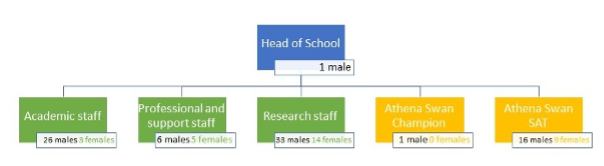
\includegraphics[width=\textwidth]{fig/schoolstructure1.png}
    %trim={<left> <lower> <right> <upper>}
    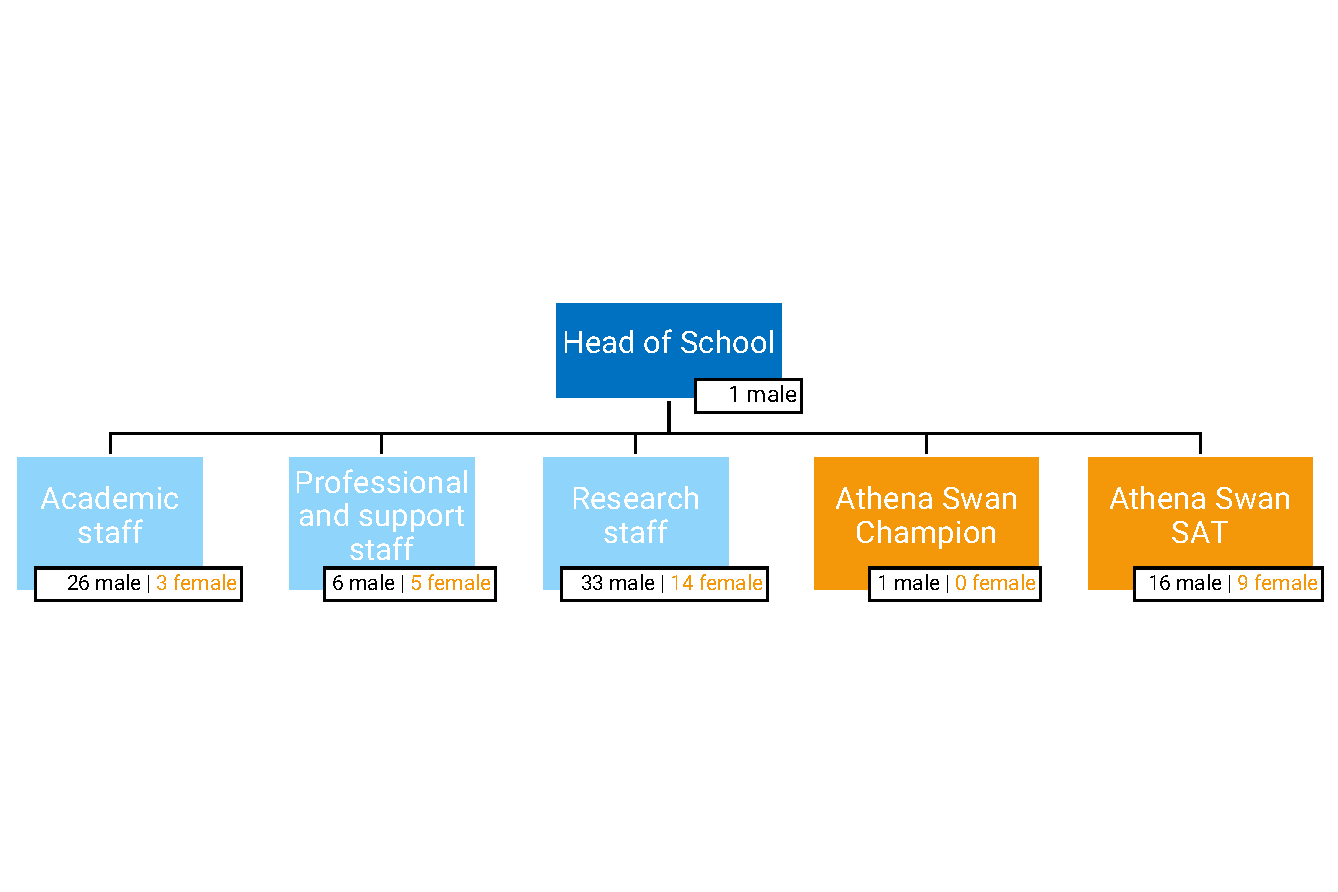
\includegraphics[trim={0 4cm 0 4cm},clip,width=\textwidth]{fig/fig1-1.pdf}
    \caption{Overall school structure based on gender and role including Athena SWAN representation}
    \label{fig:organogram}
    \todo{check update to PMS numbers}
\end{figure}



\begin{figure}[!ht]
    %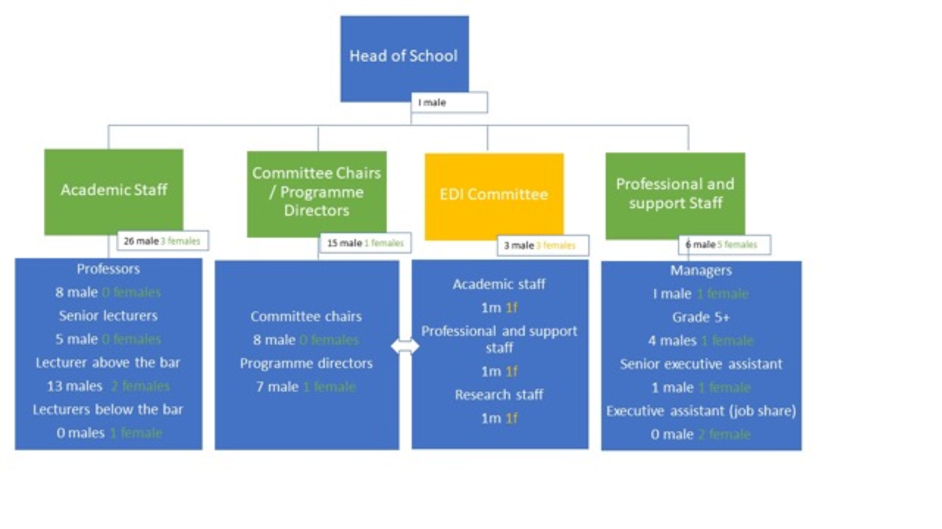
\includegraphics[width=\textwidth]{fig/fig2.pdf}
    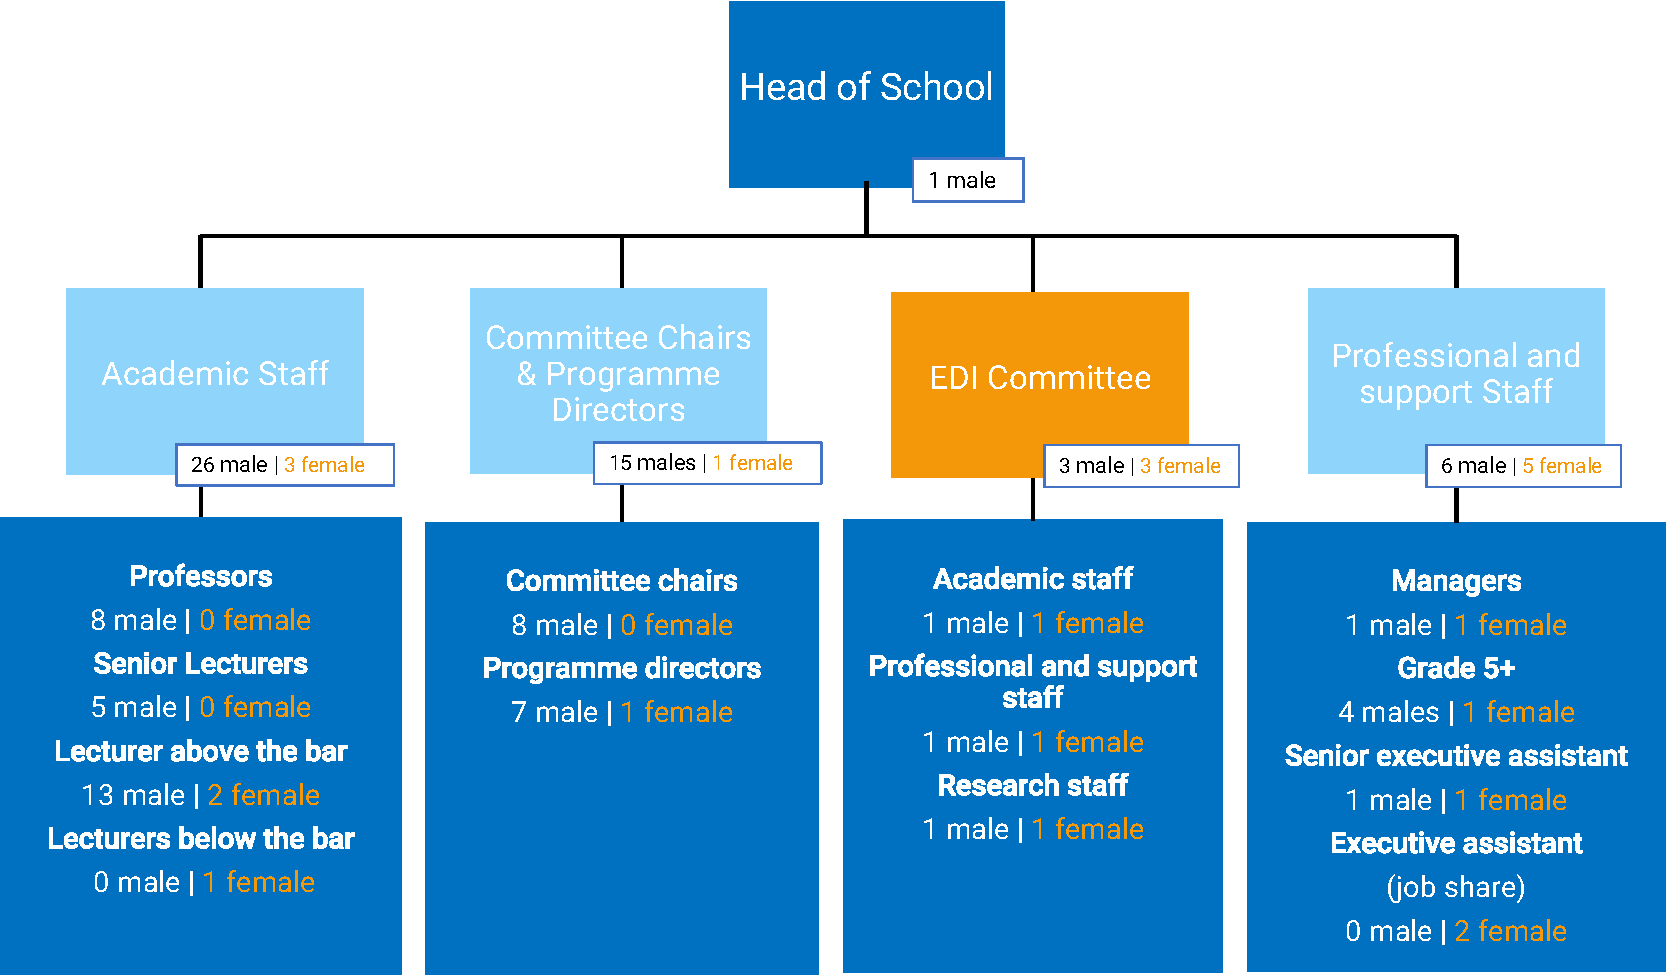
\includegraphics[width=\textwidth]{fig/fig1-2.pdf}
    \caption{Overall school management and committee structures / programme directors}
    \label{fig:schoolstructure}
    \todo{check update to PMS numbers}
\end{figure}


  

\subsubsection{Relationship between department structures and Athena SWAN structures}

Apart from the AS Champion, there have been no formal Athena SWAN structures embedded in CSIT until the establishment of the SAT in 2021. This team was composed of 25 members, reflecting the size of the CSIT. The School is regularly informed about the self-assessment activities  through a standing item on the agenda of the School's monthly meetings. 
Table~\ref{tab:activitytimeline} presents the SAT activity timeline, listing the dissemination and engagement activities within the SAT, and between the SAT and the wider community.
%\todo{The self-assessment findings were shared with all members of the school before submission and feedback was invited and accommodated.}


\subsubsection{Department support for the Athena SWAN application}
The AS activities were recognised by the \ac{HOS} in assigning administrative workload. On appointment, the Chair was relieved of other administrative obligations so that he could concentrate on coordinating the school’s AS activities. 


\subsubsection{Processes for resourcing, distributing, recognising and rewarding Athena SWAN work}
The School has only recently embarked on its AS journey, so apart from the self-assessment activities, there are currently no formal processes in place to  resource, distribute, recognise or reward AS work.
All SAT members are recognised by the \ac{HOS} for their contributions to the AS process.


\subsubsection{Resources for Implementing the Action Plan}
The School has availed of central resources provided by the university's EDI Unit for the application, which includes regular feedback and advise from the university's Athena SWAN Project Officer. It will continue to avail of all centrally available resources to support the implementation of the action plan.

Appropriate changes to the school structures will seek to support the implementation of the action plan. These systemic changes will endeavour to bring about a positive EDI culture (see Actions~\ref{action:intro:edi} and \ref{action:intro:ethos}).


\subsubsection{Other Relevant Structures and Organisation Information}
Since the School embarked on its AS journey, it has been an active member of the wider UCC EDI activities and will benefit from, and contribute to, developing best practice.


\subsubsection{Record of Gender}
All requests by staff or student to record their gender preference have been acceded to with confirmation by all data holders to record the appropriate gender.  






\section{The self-assessment process}


\subsection{Provide information on the preparation and delivery of this application by the department. This should include:}
\instr{
\begin{itemize}
\item  a description of the self-assessment team\index{self-assessment team}, including comment on the roles and responsibilities of individuals, and how these were assigned. The gender of SAT members, their professional/student role in the department, and their specific role in the SAT should be noted in a table; 
\item	information on how the chair was appointed and on what supports or resources the institution and/or department has given the chair to lead the self-assessment process; 
\item	comment on whether the self-assessment team is representative of the department, including if there is adequate representation of senior staff. 
\end{itemize}
}


\subsubsection{Description of the Self-Assessment Team}
The initial SAT  was appointed in March 2021 after an open invitation by the \ac{HOS} to all School members.
The initial 11 members were a self-selecting group, including representation from both PMS and academic staff; members were at various stages in their professional careers, and were somewhat gender balanced (see Table~\ref{tab:initialexpandedsat}).

Midway through the application process, a new Athena SWAN Charter was published, including a new application form. 
%and a new application form was created to reflect these changes.  
The SAT responded to these changed by reorganising itself into Working Groups (WGs) to better match the structure of the new application. The WG Chairs were invited by the SAT Chair. These individuals were chosen for their experience in leading teams and for their expertise in various areas, including knowledge of the UCC institutional structures. Chairs were also chosen with the intention of achieving gender balance, while taking into consideration the general gender imbalance within the school.
%a general gender imbalance within the. Despite this, only one female chair, willing to serve, could be identified.

Further, more people were invited 
to join the SAT to maximise representation and to better reflect the  diversity within the school. This expansion was done by (1) open invitation to all staff, %and all who expressed interest were accepted onto the team 
and (2) by targeting specific individuals to maximise diversity and promote inclusion; most of those who were invited, accepted. 
%1 (1M) Chair, 14 academics (3F, 11M), 7 PMSS (4F, 3M),  2 (1F, 1M) PostDocs and 3 (2F, 1M) PhD Students. 
These members were at various stages in their career, with many of the senior staff having considerable experience in the running of the school and serving on university committees.
Table~\ref{tab:initialexpandedsat} presents an overview of the initial and expanded SAT.
Table~\ref{tab:sat2c} presents details of all SAT members.
%Table~\ref{tab:initialexpandedsat} shows the composition of the initial and expanded SAT. Table~\ref{tab:sat2c} shows the gender, roles (in the school and on the SAT) of the newly constituted team. 

\begin{tabbox}{!b}
\footnotesize 
\caption{Initial and expanded SAT: Gender, leadership, and staff category}
\label{tab:initialexpandedsat}


\sisetup{
    group-digits=all,
    group-minimum-digits=4,
    group-separator = {,},
    mode=text,
    reset-text-series = false, 
    text-series-to-math = true,
    reset-text-family = false, 
    text-family-to-math = true
}   
\begin{tabular}{p{7cm}
                S[table-format=1.0]
                !{\qquad}
                S[table-format=1.0]
                !{\qquad}
                S[table-format=3.0\%]
                p{0.6cm}
                S[table-format=2.0]
                !{\qquad}
                S[table-format=2.0]
                !{\qquad}
                S[table-format=2.0\%]
                p{0.3cm}
                S[table-format=3.0\%]}
\toprule 

  & \multicolumn{3}{c}{\makecell{Initial SAT\\April 2021}} && \multicolumn{3}{c}{\makecell{Expanded SAT\\December 2021}} && {\makecell{\% by staff\\ category}}\\
  \cmidrule{2-4}\cmidrule{6-8}
  & {M} & {F} & {\%F} && {M} & {F} & {\%F} & \\
  \midrule 
 
Chair 										    & 1 & 0 & 0\% && 1 & 0 & 0\% && {n/a} \\
\hdashline
Workgroup Chairs & 0 & 0 & 0\% && 3 & 1 & 25\% && {n/a}\\
\midrule 
Academic									    & 3 & 2 & 40\% && 12 & 3 & 20\% &&52\% \\
\hdashline
Professional Management and Support Staff & 1 & 4 & 80\% && 3 & 6 & 67\% && 31\%\\
\hdashline
Research staff 								    & 0 & 0 & 0\% &&  2 & 3 & 60\% && 17\%\\
\midrule 
Total 										    & 4 & 6 & 60\% && 17 & 12 & 41\% && 100\%\\
  
\bottomrule 
\end{tabular}

\end{tabbox}



\begingroup
\newcommand{\mycolwidth}{3.2cm}
\setlength{\tabcolsep}{7pt} % Default value: 6pt



% \colorbox{SwanOrange!10}{
%     \begin{minipage}{14.3cm}
%     \begin{table}[H]
%     \footnotesize 
%     \caption{Athena SWAN Self Assessment Team}
%     \label{tab:sat2c}
%     \begin{tabular}{@{}p{\mycolwidth}p{\mycolwidth}p{\mycolwidth}p{\mycolwidth}@{}}
   
%     \multicolumn{4}{@{}l}{\large\textbf{Athena SWAN Self Assessment Team}}\\

%     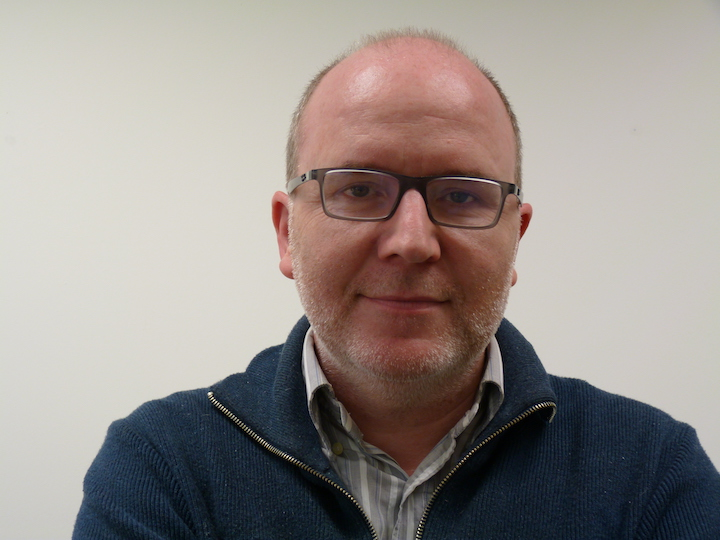
\includegraphics[width=\mycolwidth]{img/DavidOB.JPG}
%     \makecell{John Morrisson | M\\
%     Professor\\
%     \textbf{SAT Chair}}
% &

%     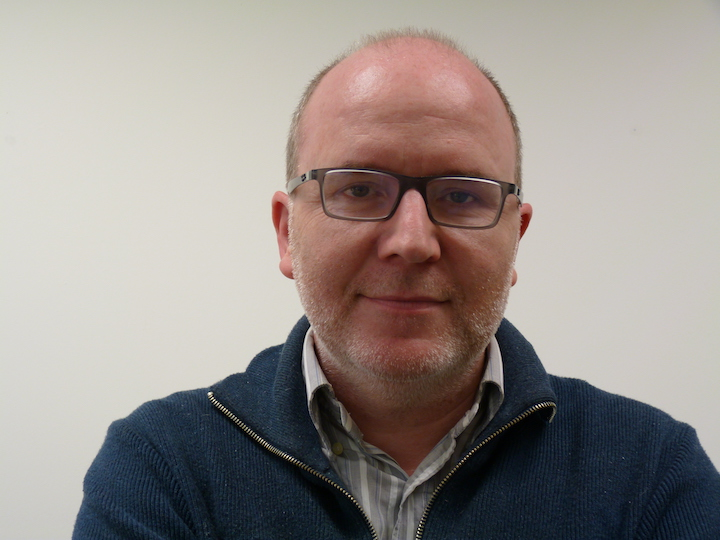
\includegraphics[width=\mycolwidth]{img/DavidOB.JPG}
%     \makecell{Klaas-Jan Stol | M\\
%     Lecturer\\
%     WG Liaison}\\

%     \end{tabular}
%     \end{table}
%     \end{minipage}
% }



\colorbox{orangebg}{
    \begin{minipage}{14.2cm}
    \vspace{-4mm}
    \begin{table}[H]
    \singlespacing
    \caption{Athena SWAN Self Assessment Team}
    \label{tab:sat2c}
    
    \footnotesize 
    \begin{tabular}{@{}
    p{\mycolwidth}p{\mycolwidth}p{\mycolwidth}p{\mycolwidth}@{}}

    %\multicolumn{4}{@{}l}{\textit{Continued from previous page}}\\
    \toprule 
    
    \multicolumn{4}{@{}l}{\textbf{Athena SWAN Self Assessment Team}}\\
    
    
    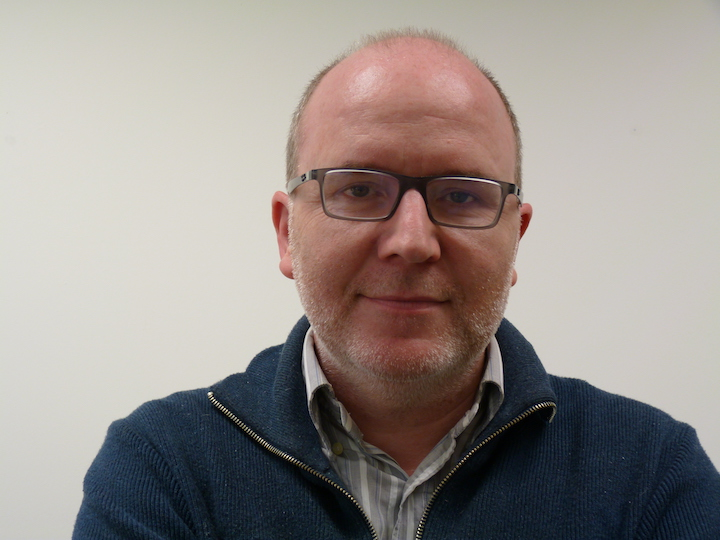
\includegraphics[width=\mycolwidth]{img/DavidOB.JPG}
    \makecell{John Morrisson | M\\
    Professor\\
    \textbf{SAT Chair}}
&
    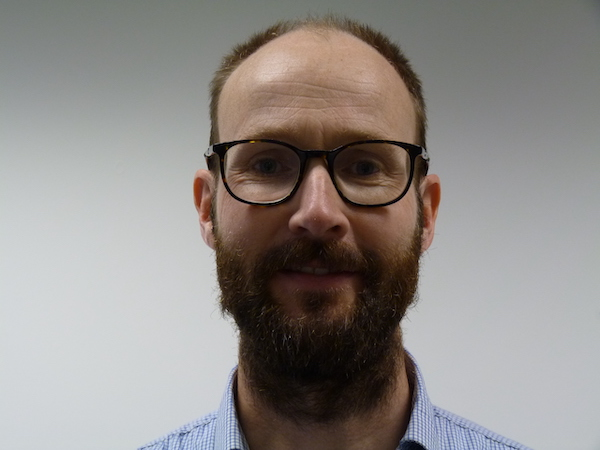
\includegraphics[width=\mycolwidth]{img/klaas.JPG}
    \makecell{Klaas-Jan Stol | M\\
    Lecturer\\
    WG Liaison}\\

%%%%%%%%%%%%%%%%%%%%%%%%%%%%%%%%%%%%%%%%%%%%%%%

    

%%%%%%%%%%%%%%%%%%%%%%%%%%%%%%%%%%%%%%%% WG 2

   

%%%%%%%%%%%%%%%%%%%%%%%%%%%%%%%%%%%%%%%%%%%%%%%%%%%%%%%%%%%

%     \multicolumn{4}{@{}l}{\large\textbf{Work Group 3: Professional, Management and Support Careers}}\\

%     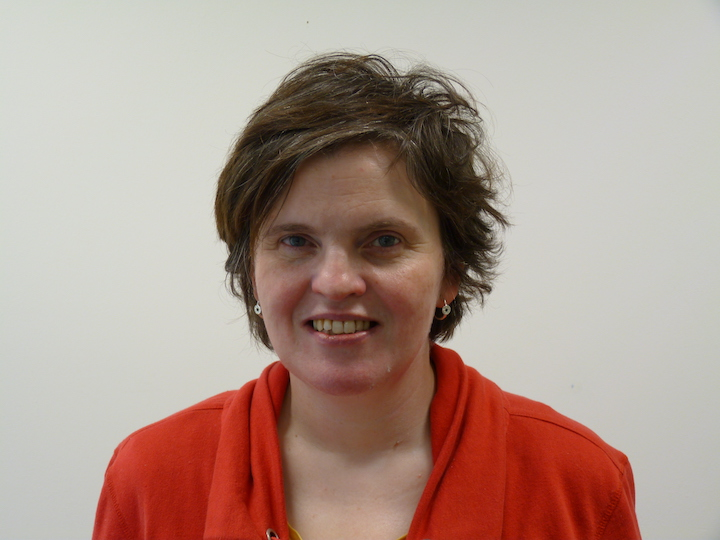
\includegraphics[width=\mycolwidth]{img/Julie.JPG}
%     \makecell{Aisling O'Driscoll | F\\
%     Lecturer | 
%     \textbf{WG3 Lead}\\
%     Coordinator CK401}
% &
%     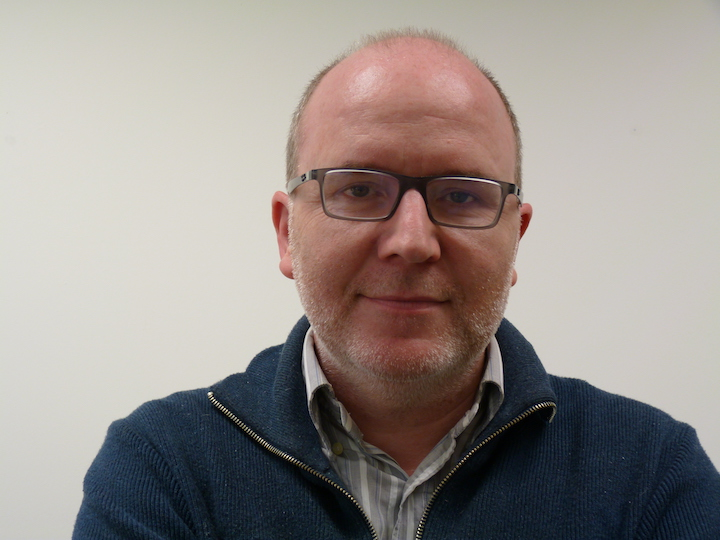
\includegraphics[width=\mycolwidth]{img/DavidOB.JPG}
%     \makecell{David O'Byrne | M\\
%     Computer Systems\\
%     Manager}
% &
%     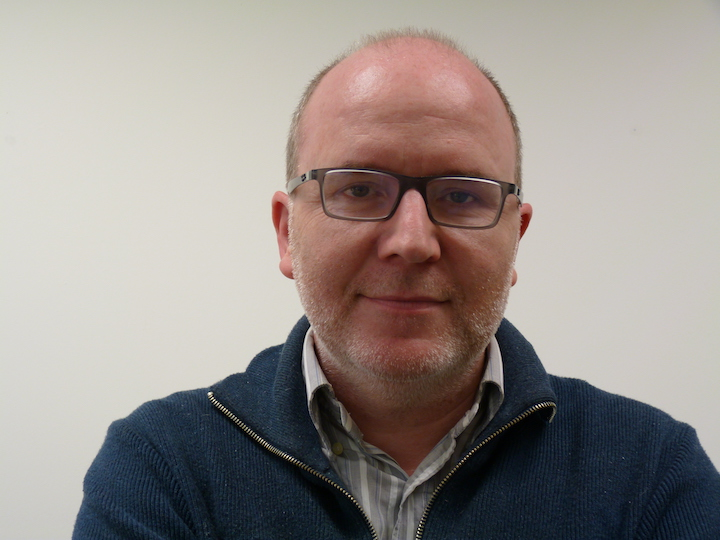
\includegraphics[width=\mycolwidth]{img/DavidOB.JPG}
%     \makecell{Adrian O'Riordan | M\\
%     Lecturer}
% &
%     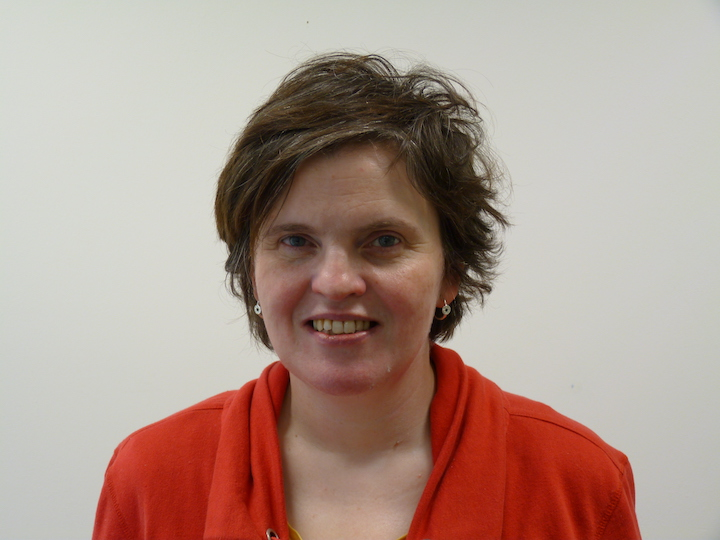
\includegraphics[width=\mycolwidth]{img/Julie.JPG}
%     \makecell{Youngsin O'S\'{e} | F\\
%     Administrator}\\

    \end{tabular}
    \end{table}
    
    \begin{flushright}
    {\sffamily \textit{Continued on next page} }
    \end{flushright}
    \end{minipage}
}


% %%%%%%%%%%%%%%%%%%%%%%%%%%%%%%%%%%%%%%%%%%%%%%%%%%%%%%%%%%%%%

\colorbox{orangebg}{
    \begin{minipage}{14.2cm}
    {\sffamily \textit{Continued from previous page}}\\
    \begin{table}[H]
    \footnotesize 
    
    \begin{tabular}{@{}p{\mycolwidth}p{\mycolwidth}p{\mycolwidth}p{\mycolwidth}@{}}

    %\multicolumn{4}{@{}l}{\textit{Continued from previous page}}\\

\multicolumn{4}{@{}l}{\textbf{Work Group 1: Department and Its Context}}\\

    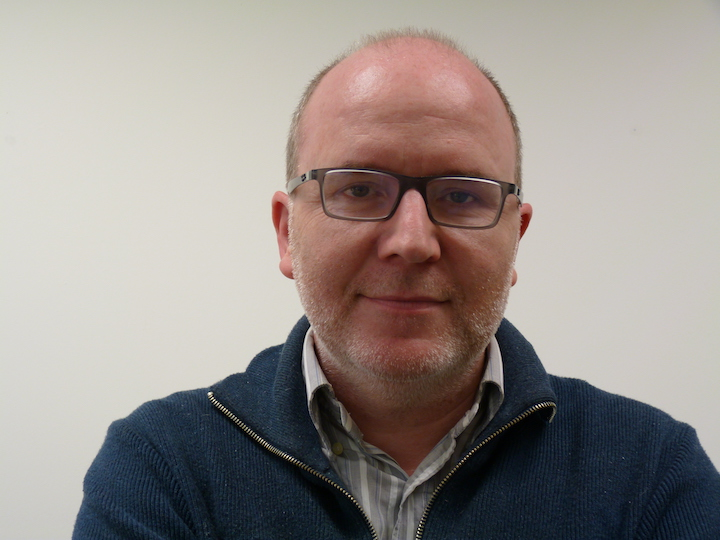
\includegraphics[width=\mycolwidth]{img/DavidOB.JPG}
    \makecell{Kieran Herley | M\\
    Lecturer | \textbf{WG1 Leader}\\
    Chair Teaching\\Committee}
&
    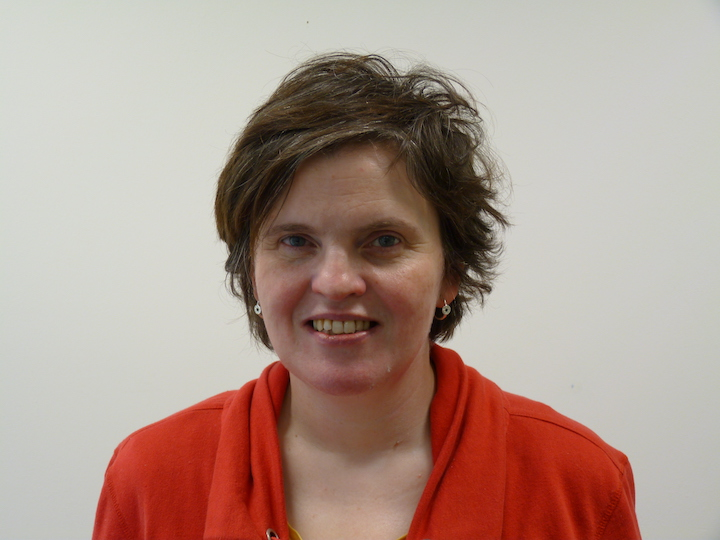
\includegraphics[width=\mycolwidth]{img/Julie.JPG}
    \makecell{Derbhile Timon | F\\
    School Manager}
&
    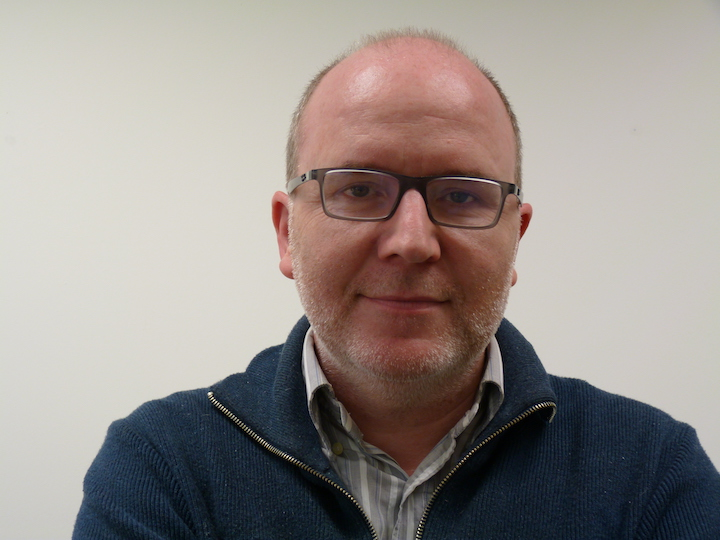
\includegraphics[width=\mycolwidth]{img/DavidOB.JPG}
    \makecell{John O'Mullane | M\\
    Lecturer}
&
    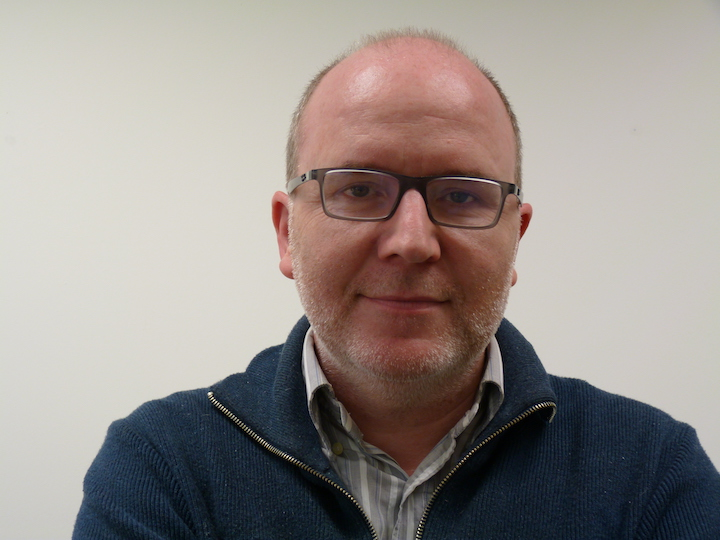
\includegraphics[width=\mycolwidth]{img/DavidOB.JPG}
    \makecell{Martin Moriarty | M\\
    IT Administrator}\\
    \\
    
 \multicolumn{4}{@{}l}{\textbf{Work Group 2: Academic and Research Careers}}\\

    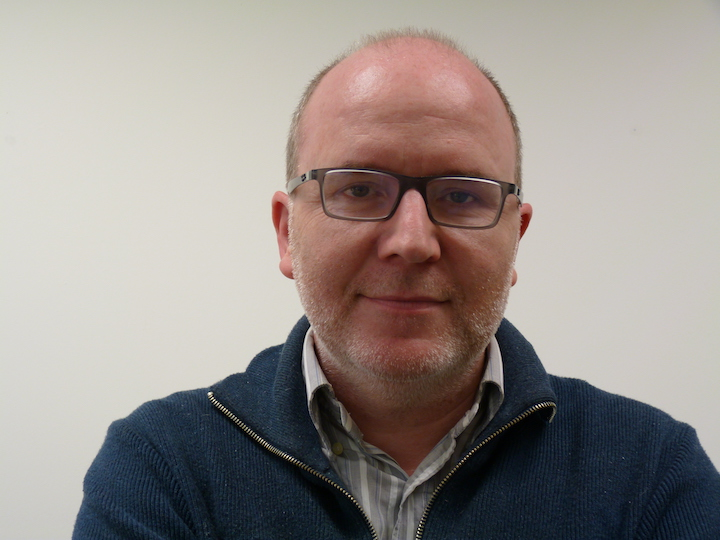
\includegraphics[width=\mycolwidth]{img/DavidOB.JPG}
    \makecell{Dirk Pesch | M\\
    Professor | 
    \textbf{WG2 Lead}}
&
    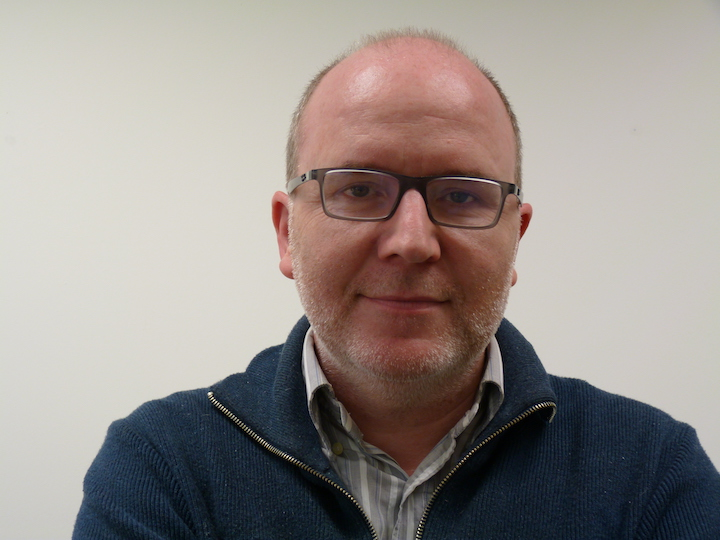
\includegraphics[width=\mycolwidth]{img/DavidOB.JPG}
    \makecell{Jason Quinlan | M\\
    Lecturer}
&
    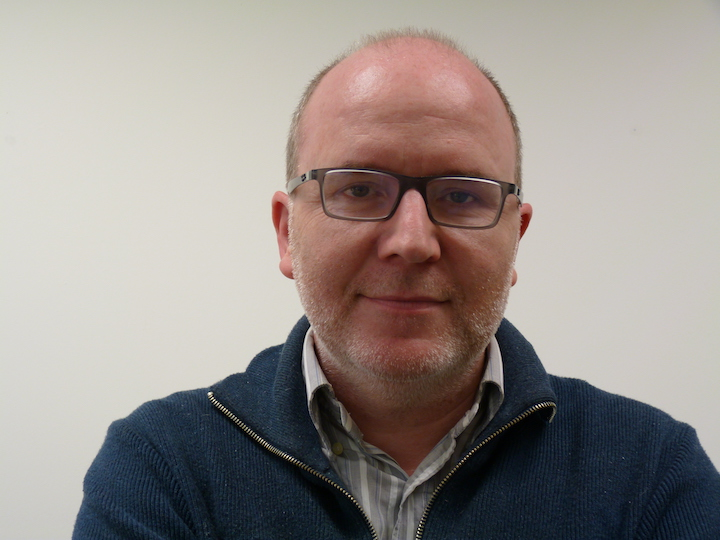
\includegraphics[width=\mycolwidth]{img/DavidOB.JPG}
    \makecell{Andrea Visentin | M\\
    Lecturer}
&
    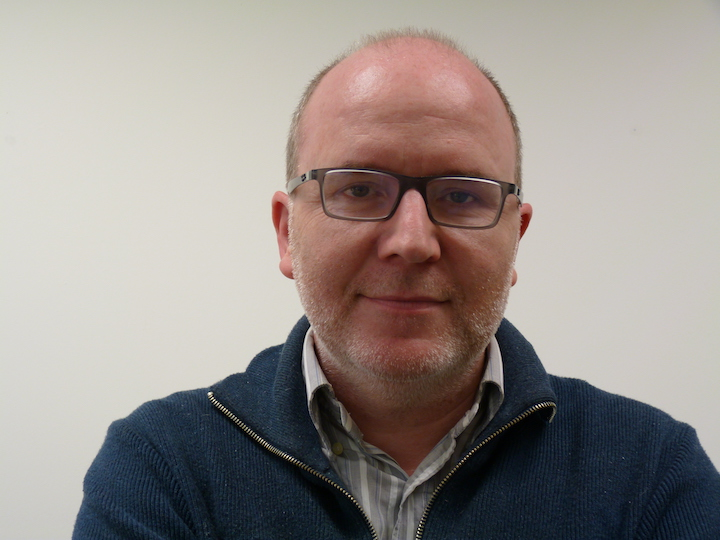
\includegraphics[width=\mycolwidth]{img/DavidOB.JPG}
    \makecell{Barry O'Sullivan | M\\
    Professor}\\

    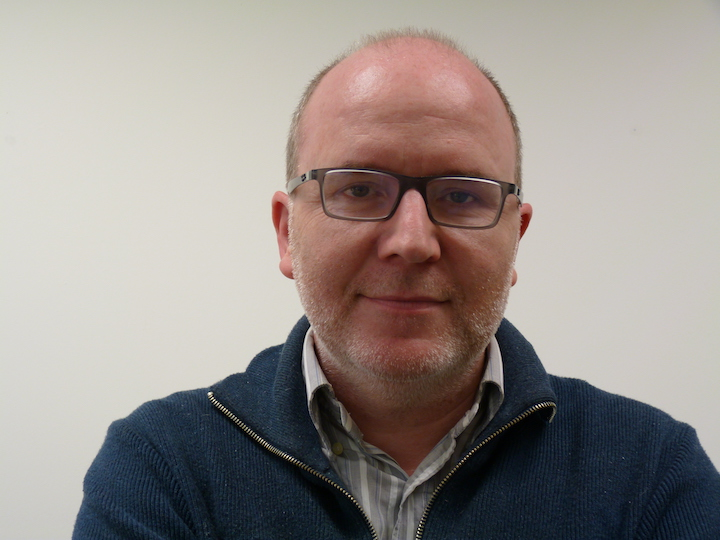
\includegraphics[width=\mycolwidth]{img/DavidOB.JPG}
    \makecell{Md. Noor-A-Rahim | M\\
    Senior Postdoc}
&
    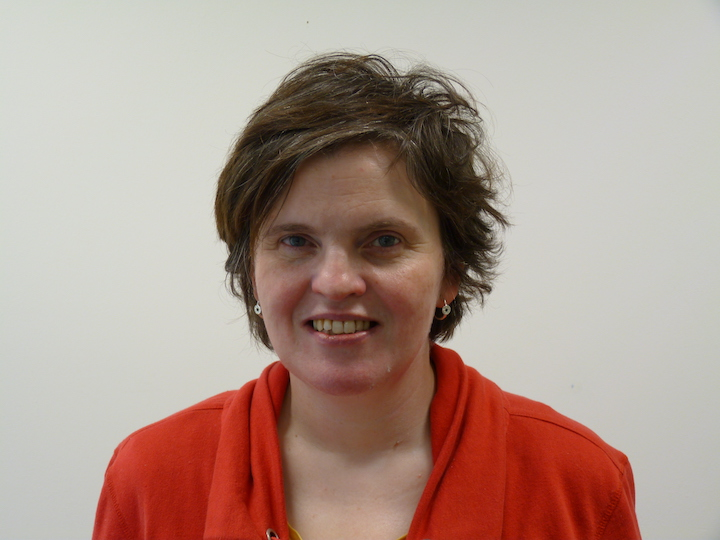
\includegraphics[width=\mycolwidth]{img/Julie.JPG}
    \makecell{Buvana Ganesh | F\\
    PhD candidate}
&
    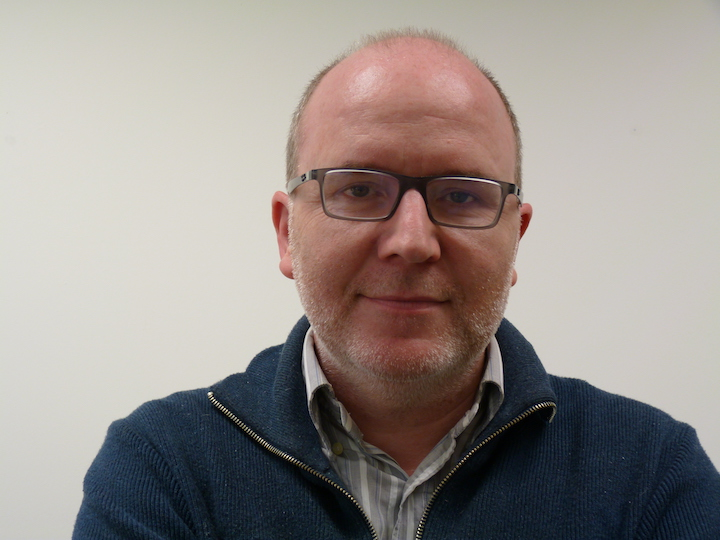
\includegraphics[width=\mycolwidth]{img/DavidOB.JPG}
    \makecell{Vlad Ionescu | M\\
    PhD candidate}
&
    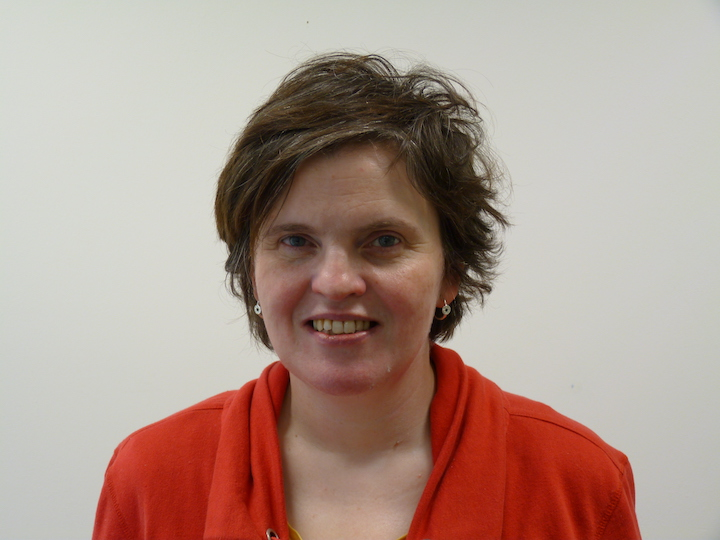
\includegraphics[width=\mycolwidth]{img/Julie.JPG}
    \makecell{Begum Genk | F\\
    Postdoc}\\

    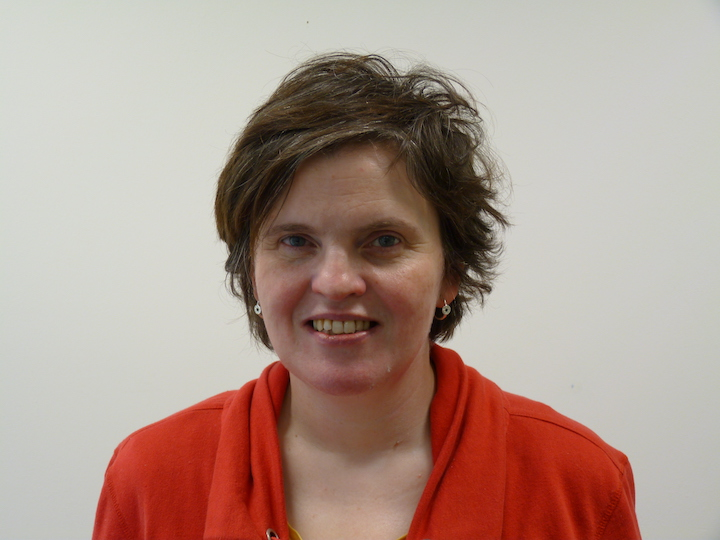
\includegraphics[width=\mycolwidth]{img/Julie.JPG}
    \makecell{Rosane Minghim  | F\\
    Lecturer}\\
    




    
    \end{tabular}
    \end{table}
    \end{minipage}
}

\colorbox{orangebg}{
    \begin{minipage}{14.2cm}
    {\sffamily \textit{Continued from previous page}}\\
    \begin{table}[H]
    \footnotesize 
    
    \begin{tabular}{@{}p{\mycolwidth}p{\mycolwidth}p{\mycolwidth}p{\mycolwidth}@{}}
    
        \multicolumn{4}{@{}l}{\textbf{Work Group 3: Professional, Management and Support Careers}}\\

    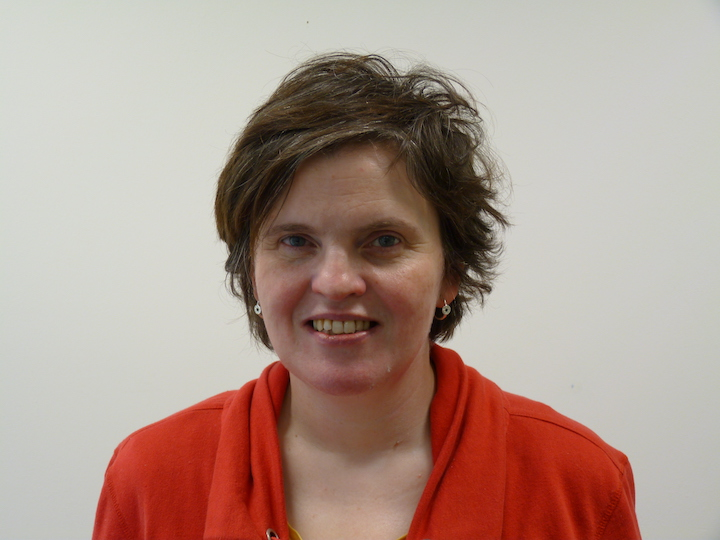
\includegraphics[width=\mycolwidth]{img/Julie.JPG}
    \makecell{Aisling O'Driscoll | F\\
    Lecturer | 
    \textbf{WG3 Lead}\\
    Coordinator CK401}
&
    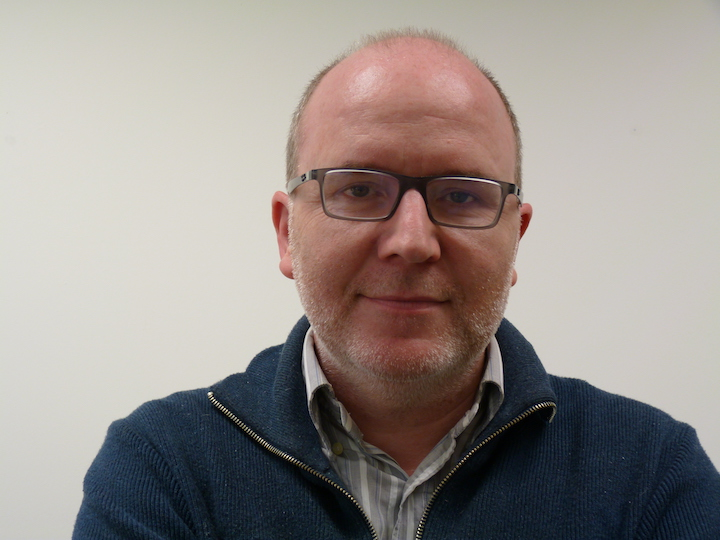
\includegraphics[width=\mycolwidth]{img/DavidOB.JPG}
    \makecell{David O'Byrne | M\\
    Computer Systems\\
    Manager}
&
    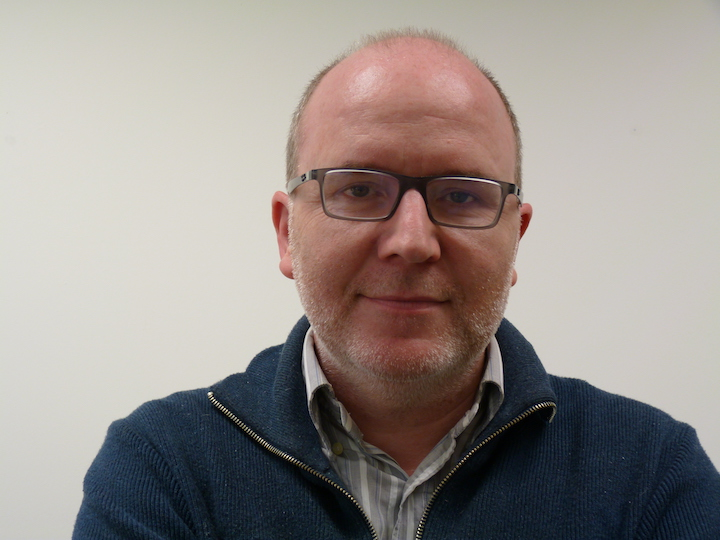
\includegraphics[width=\mycolwidth]{img/DavidOB.JPG}
    \makecell{Adrian O'Riordan | M\\
    Lecturer}
&
    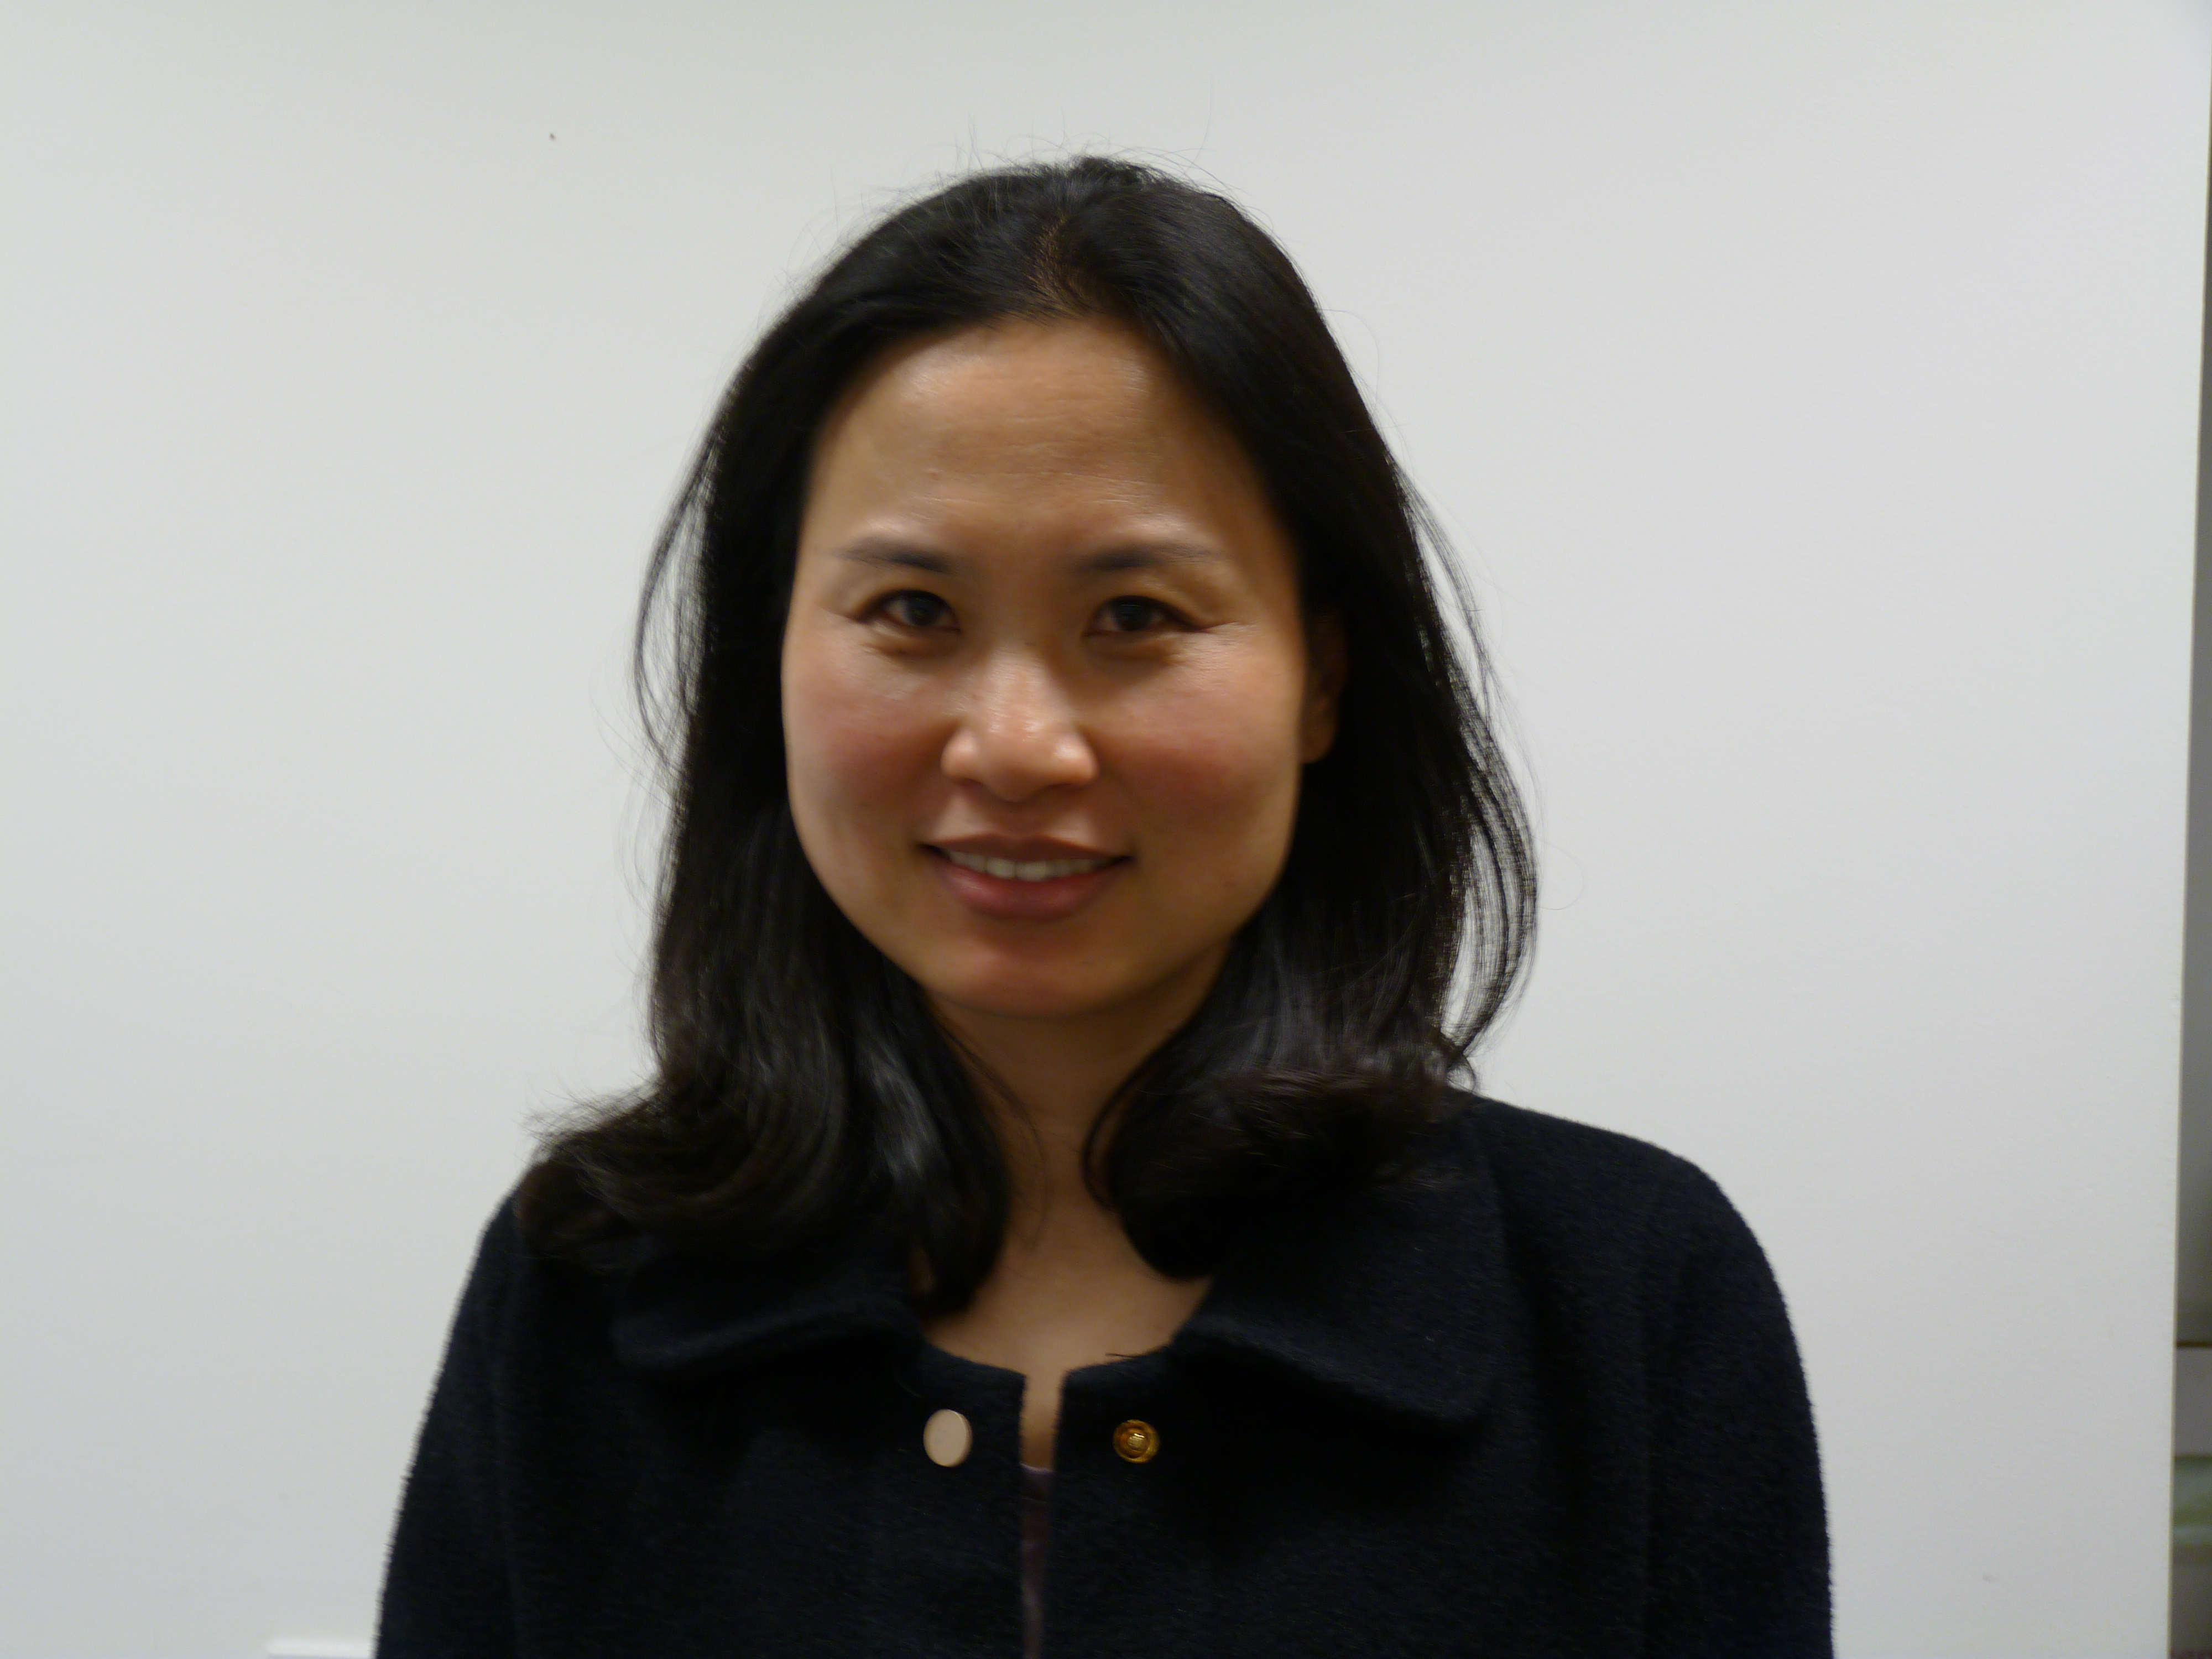
\includegraphics[width=\mycolwidth]{img/P1110828.JPG}
    \makecell{Youngsin O'S\'{e} | F\\
    Administrator}\\
    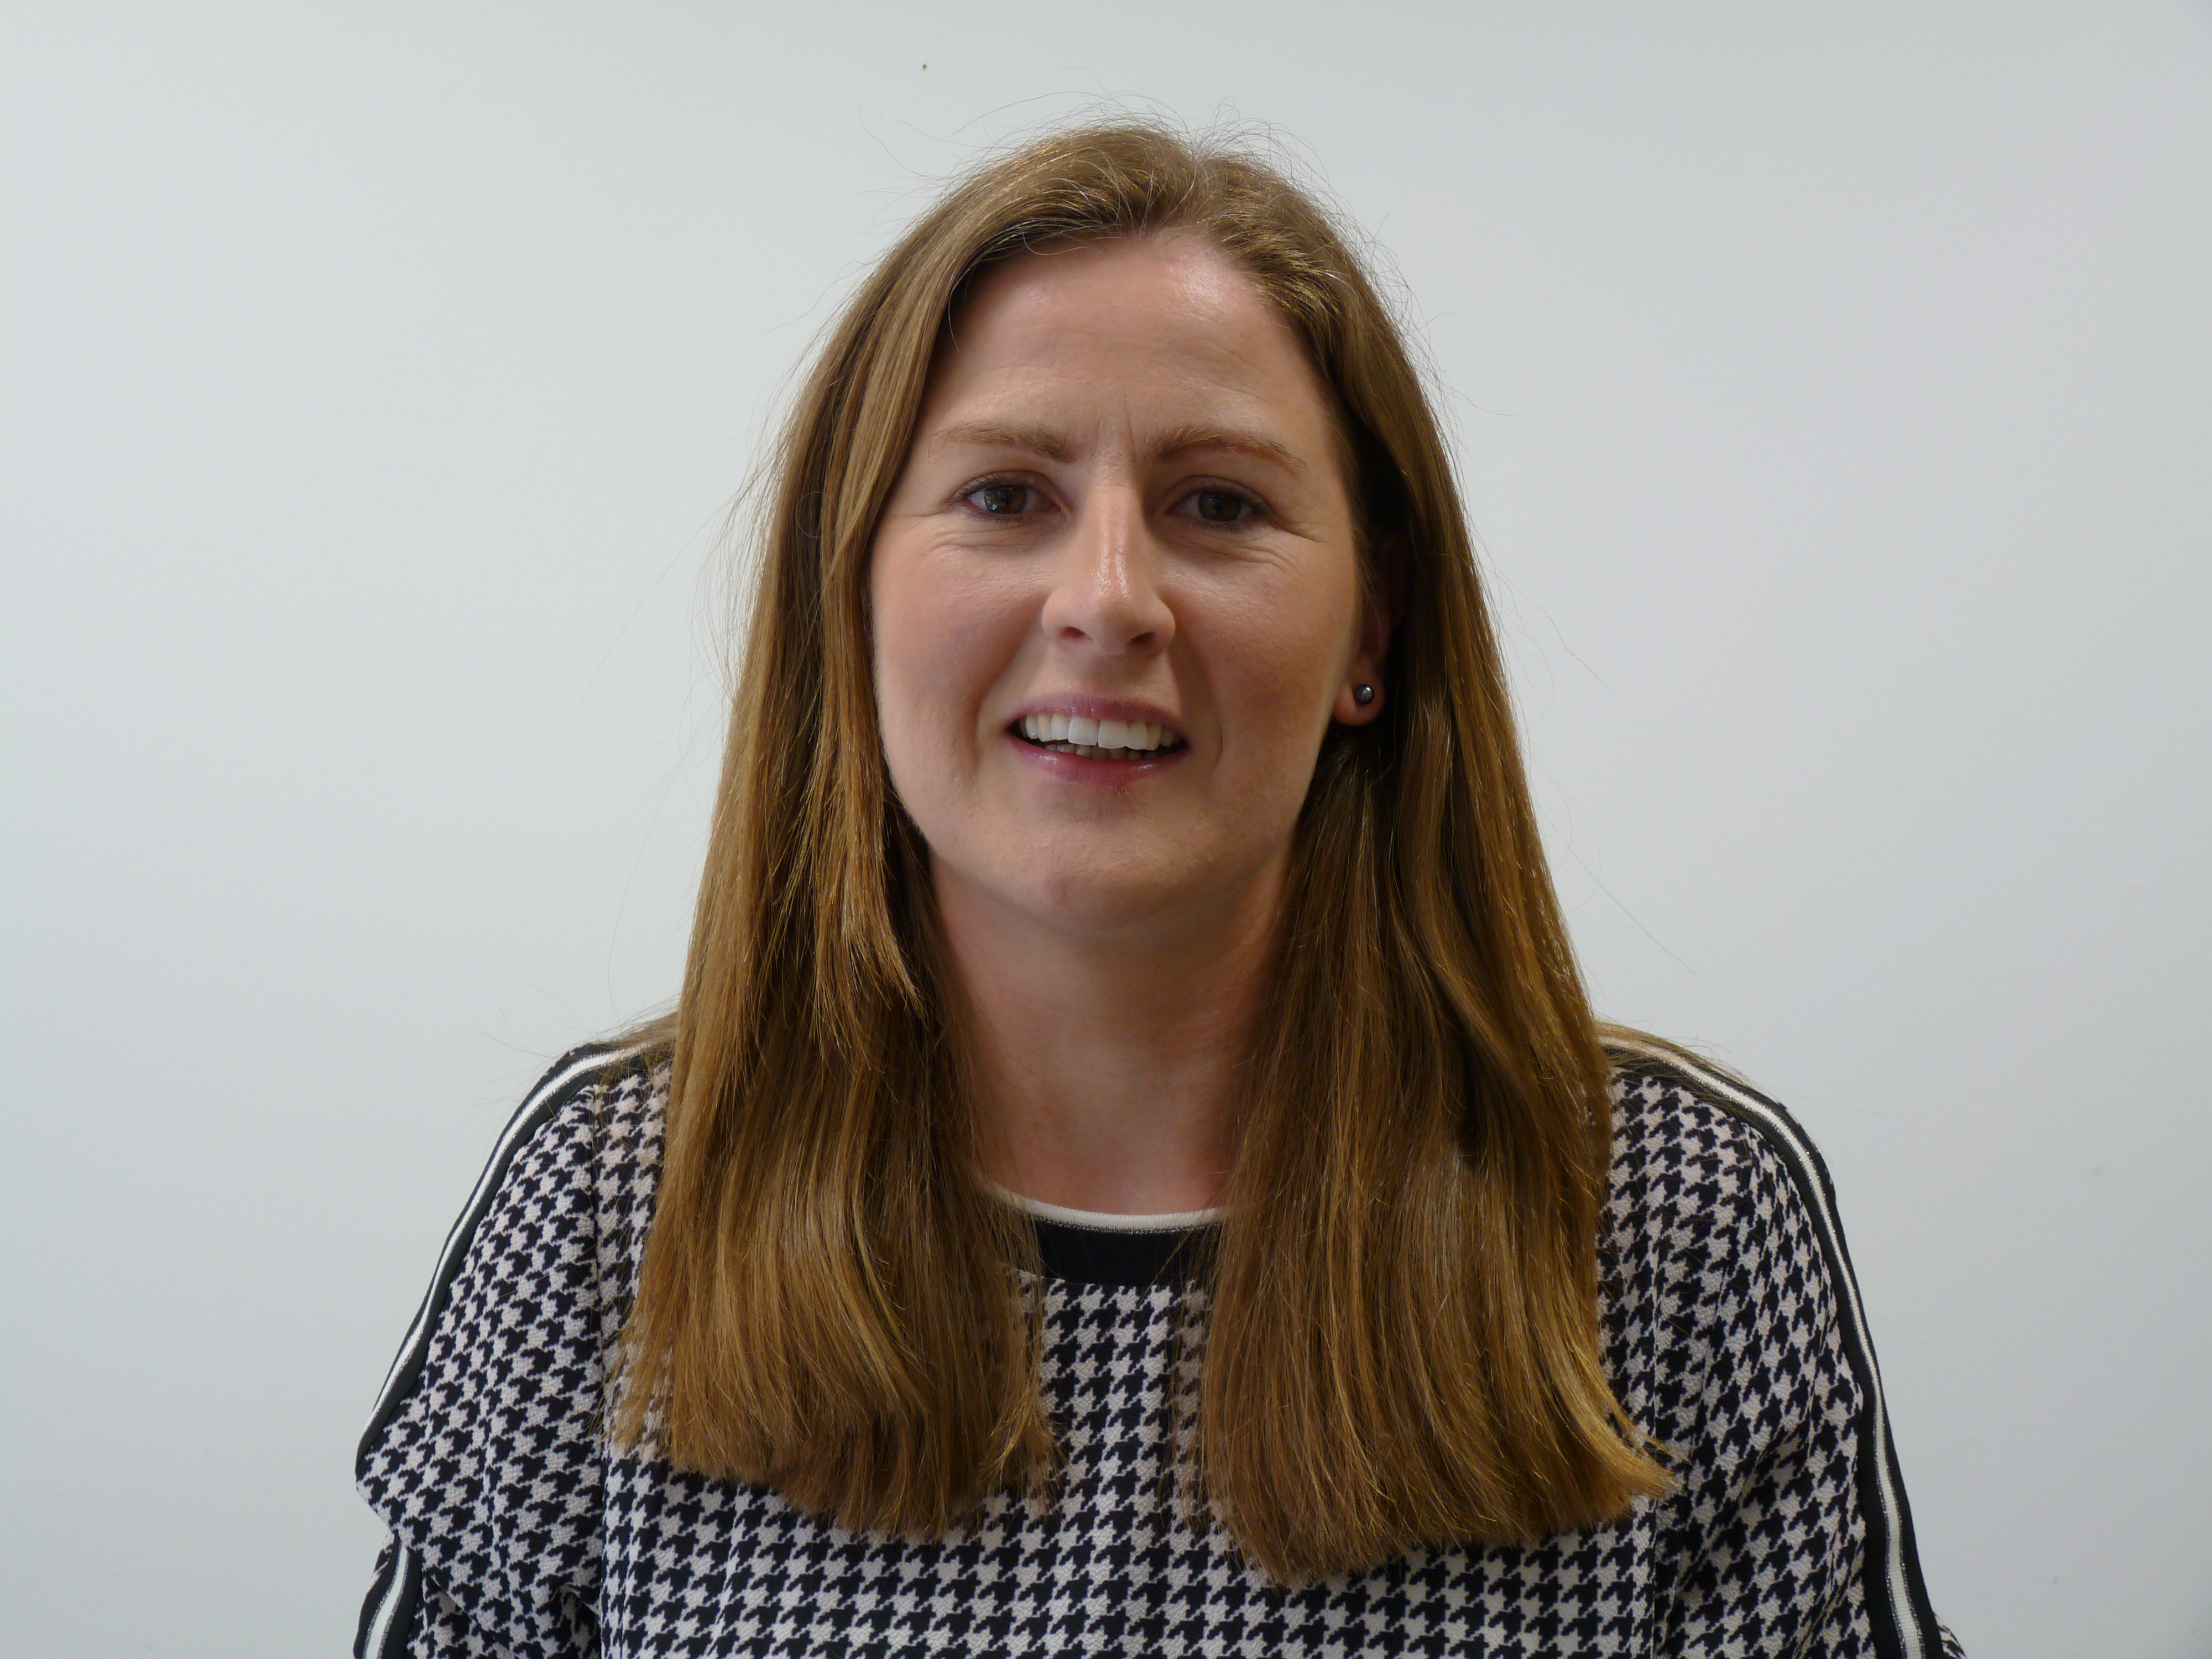
\includegraphics[width=\mycolwidth]{img/P1110826.JPG}
    \makecell{Eleanor O'Riordan | F\\
    Administrator}
&
    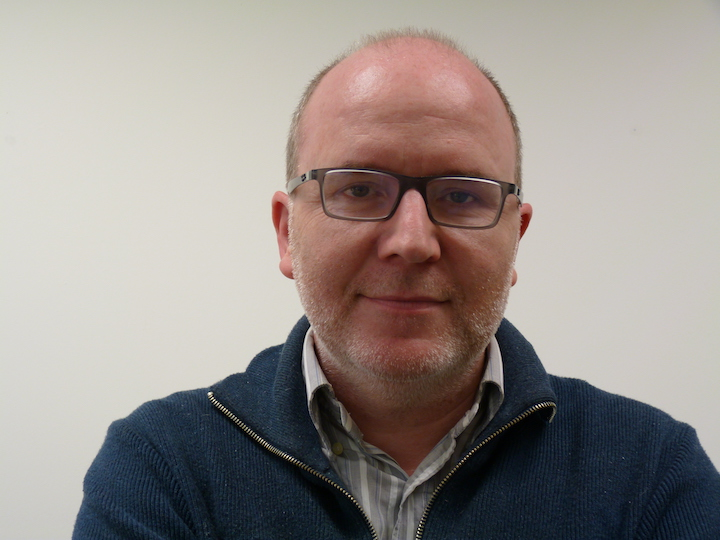
\includegraphics[width=\mycolwidth]{img/DavidOB.JPG}
    \makecell{James Duggan | M\\
    Administrator}\\
    \\
    
    \multicolumn{4}{@{}l}{\textbf{Work Group 4: Inclusion and Belonging}}\\

    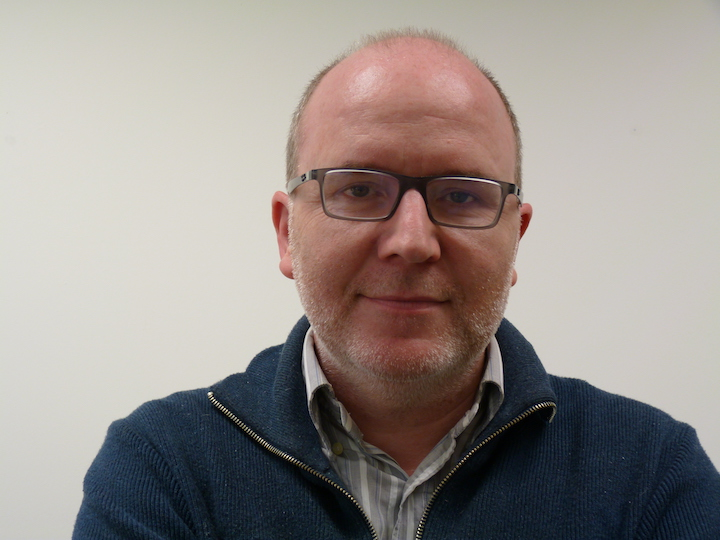
\includegraphics[width=\mycolwidth]{img/DavidOB.JPG}
    \makecell{Paolo Palmieri | M\\
    Lecturer |
    \textbf{WG4 Lead}}
&
    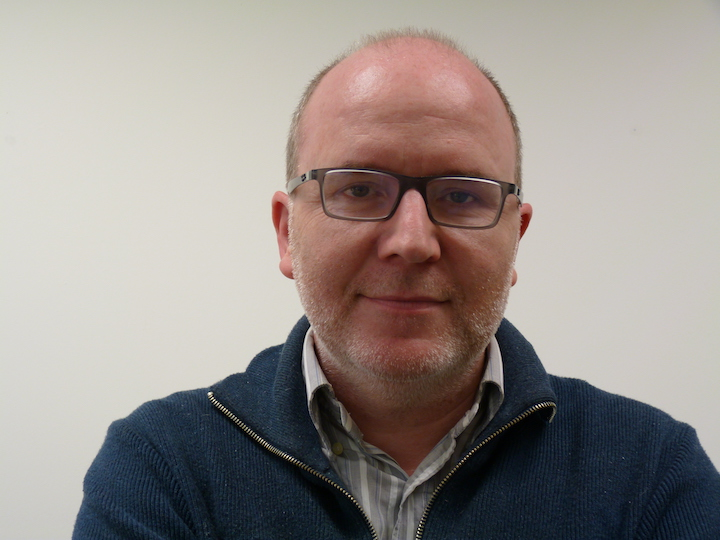
\includegraphics[width=\mycolwidth]{img/DavidOB.JPG}
    \makecell{Ahmed Zahran | M\\
    Lecturer}
&
    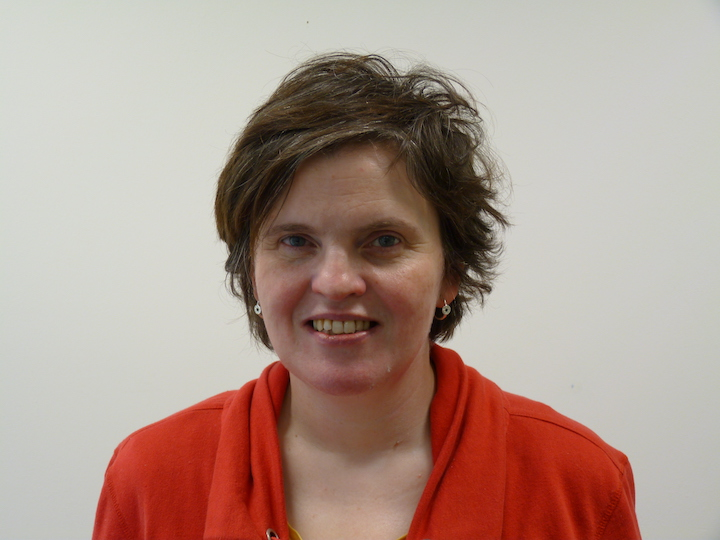
\includegraphics[width=\mycolwidth]{img/Julie.JPG}
    \makecell{Andrea Balogh | F\\
    PhD candidate}
&
    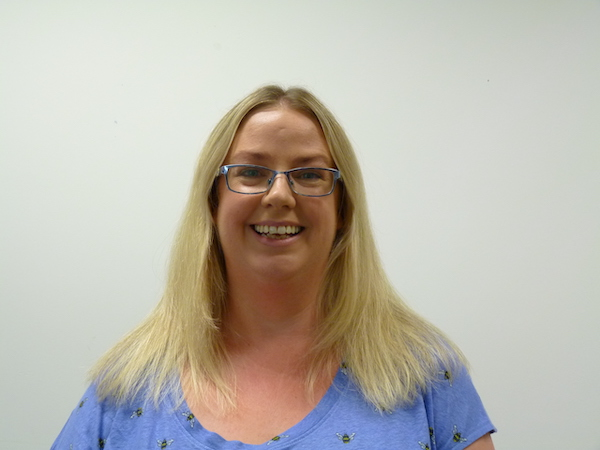
\includegraphics[width=\mycolwidth]{img/joanne.JPG}
    \makecell{Joanne Murphy | F\\
    Administrator}\\

    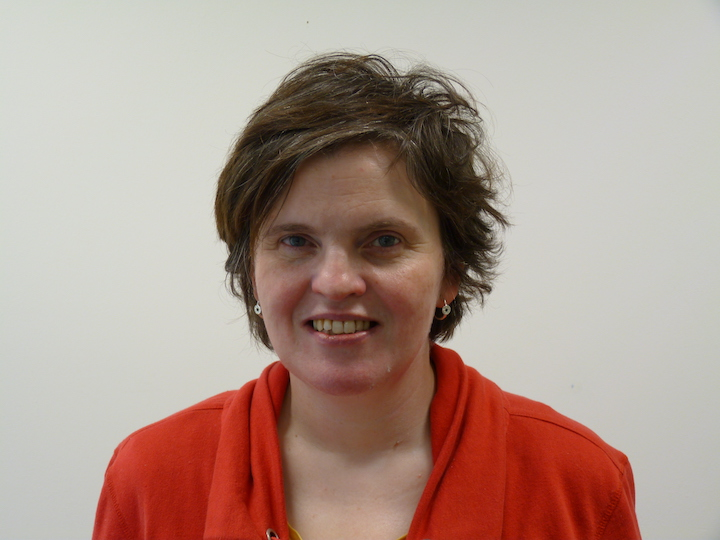
\includegraphics[width=\mycolwidth]{img/Julie.JPG}
    \makecell{Laura Maye | F\\
    Lecturer}
&
    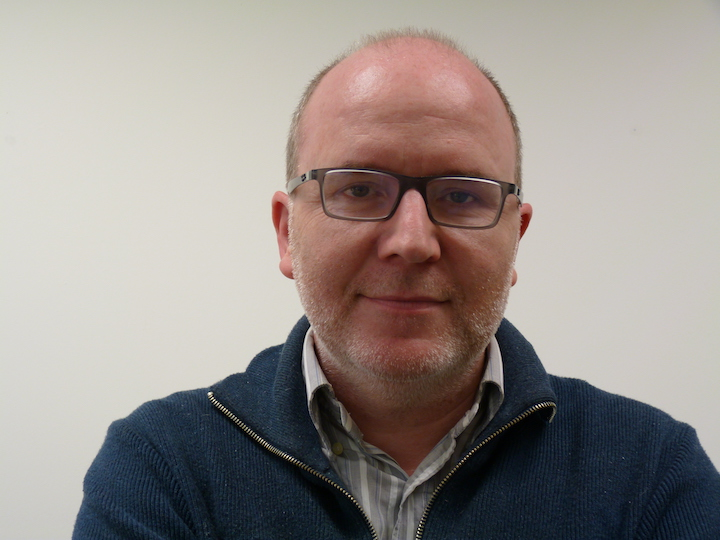
\includegraphics[width=\mycolwidth]{img/DavidOB.JPG}
    \makecell{Sabin Tabirca | M\\
    Senior Lecturer}\\

    \bottomrule 
    
    \end{tabular}
    \end{table}
    \end{minipage}
}


\endgroup 


\subsubsection{Appointment of the SAT Chair}
Following an open invitation, in March 2021, 
%in which all staff were invited to express interest in serving as the SAT Chair.  The 
the \ac{HOS} appointed a senior staff member to the position, reflecting the commitment of the School to AS process. 
%Recognising the importance and considerable effort of the role, the SAT Chair was relieved 
%This commitment was strengthened by also relieving the SAT Chair 
%of other administrative roles to concentrate on the process. 


\subsubsection{Representation on the SAT}

Both of the female academic staff members and over 50\% of female PMS staff were members of the SAT. 
%Given the large number of research staff and students in the School, it was not feasible to have a proportional representation from these groups. However, 66\% of the SAT members from these cohorts were female. 
In total 37\% of the SAT were female, which is greater than the percentage of females in the School as a whole.
Six members of the SAT were senior staff, including 3 Professors, 1 Senior Lecturer, 1 Systems Administration Manager, and 1 School Manager. 
%The senior staff are represented on the SAT by 3 Professors, 1 Senior Lecturer, 1 Systems Administration Manager and 1 School Manager (1F). 
%Currently the School has no senior female academic members. 


\subsection{Provide information on the preparation and delivery of this application by the department. This should include:}
\instr{
\begin{itemize}
\item an overview of the approach taken to evidence-gathering and analysis. Details of consultation response rates, disaggregated by gender, should be provided;
\item	information on plans for evaluating progress, including action plan implementation, over the coming four-year period. This should make reference to how often the SAT will meet, and how SAT succession and turnover will be planned and managed; 
\item	information on how the findings and activity of the self-assessment team are, and will continue to be, communicated to senior management and the wider department.
\end{itemize}
}


\subsubsection{Approach to evidence-gathering and analysis}

%The School began the process of applying for Athena SWAN (AS) certification in March 2021. 
The SAT held several orientation meetings in April and May of 2021 to understand the scope of the AS process and to share ideas and experiences. Meetings were also held between UCC's EDI unit and the SAT Chair. 
%The substance of these meetings was shared with the SAT and were invaluable in communicating the institutional ethos and the supports available. They also helped to guide the SAT, to outline practical activities, and to set priorities.

At the time the SAT was formed, Covid-19 restrictions were in full force. A dedicated Microsoft Teams team was created for the SAT, and all SAT meetings were conducted online.
%The SAT was formed at a challenging time. Covid-19 restrictions were in full force, SAT meetings were online, 
While staff were under pressure to meet the challenges of working remotely, much progress was made, and, under the guidance of the EDI unit, the committee created a staff survey to provide insight into relevant attitudes and experiences of staff within the school.

The SAT began working with the standard survey provided by the EDI unit. This was augmented by the SAT to the reflect the profile of the school and to maximise opportunities for staff to provide written feedback, highlighting issues and experiences. 
Where practical, questions in the standard survey were augmented with a text box, inviting in-depth feedback and opinions. 
In addition, questions were added on parental leave, experiences of new staff and experiences of staff from under-represented groups. Finally, large portions of the survey were replicated in a dedicated section to capture experiences during the Covid-19 restrictions. This was done to capture how well the school responded to the needs of staff when faced with the pressure of external challenges. The survey was officially launched by the \ac{HOS} at the end of June 2021 and remained open until July 14th, 2021. %The survey was managed by the EDI unit. 
There were 56 responses, giving a participation rate of 62\%.  The response rates by gender for academic and PMS reflect the gender balance in the school. Tables~\ref{tab:response:bygender} and \ref{tab:response:byrole} present the response rates by gender and by role, respectively.


\begin{tabbox}{!t}

\caption{Survey response by gender, compared to total School staff count and gender distribution, and response rate by gender}
\label{tab:response:bygender}
\sisetup{
    group-digits=all,
    group-minimum-digits=4,
    group-separator = {,},
    table-format=4.1,
    mode=text,
    reset-text-series = false, 
    text-series-to-math = true,
    reset-text-family = false, 
    text-family-to-math = true
}
\footnotesize   
\begin{tabular}{p{4.5cm} 
                !{\qquad}
                S[table-format=2.0]
                !{\quad}
                S[table-format=2.1\%]
                p{0.5cm}
                S[table-format=2.0\%]                 
                !{\quad}
                S[table-format=2.1\%] 
                !{\qquad}
                S[table-format=2.1\%]                 
                } 

\toprule 
    & \multicolumn{2}{c}{\makecell{Gender representation\\of survey respondents}} 
    &
    & \multicolumn{2}{c}{\makecell{Gender representation\\of all staff School of CSIT}} 
    & {\multirow{2}{2cm}{\makecell{Overall\\Response\\rate}}}\\
    \cmidrule{2-3}\cmidrule{5-6}
Gender & {Count} & {\%} && {Count} & {\%} &  \\ 
\midrule 
Female & 16 & 28.6\% &&  19 & 23.5\% & 84.2\%\\
\hdashline
Male & 37 & 66.1\% && 62 &  76.5\% &59.7\%\\
\hdashline
Prefer not to say & 3 & 5.4\% && {n/a} & {n/a} & {n/a}\\
\midrule 
Total & 56 & 100.0\% && 81 & 100.0\% &69.1\%\\
\bottomrule 
\end{tabular}


\end{tabbox}


% \begin{SCfigure}[10][!ht]
% \hspace{-3pt}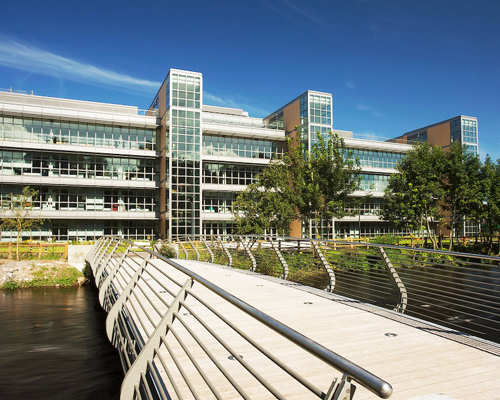
\includegraphics[width=3in]{img/WGB.jpg}
% \caption{Western Gateway Building: home to CSIT}
% \label{fig:wgb}
% \end{SCfigure}


\begin{tabbox}{!th}
\caption{Survey response by role}
\label{tab:response:byrole}
\sisetup{
    group-digits=all,
    group-minimum-digits=4,
    group-separator = {,},
    table-format=4.1,
    mode=text,
    reset-text-series = false, 
    text-series-to-math = true,
    reset-text-family = false, 
    text-family-to-math = true
}
\footnotesize   
\begin{tabular}{p{6.0cm} 
                !{\qquad}
                S[table-format=2.0]
                !{\quad}
                S[table-format=2.1\%]
                p{0.5cm}                
                S[table-format=2.0]
                !{\quad}
                S[table-format=3.2\%]
                p{0.5cm}                
                S[table-format=2.0]
                !{\quad}
                S[table-format=3.1\%]
                }

\toprule 
&\multicolumn{2}{c}{\makecell{Total survey\\ responses}}&&\multicolumn{2}{c}{\makecell{Female survey\\responses}}&&\multicolumn{2}{c}{\makecell{Male survey\\ responses}}\\
\cmidrule{2-3}\cmidrule{5-6}\cmidrule{8-9}
Category & {Count} & {\%} && {Count} & {\%} && {Count} & {\%}\\
\midrule 
Professional, Managerial and Support Staff & 14 & 25.0\% && 8 & 50.00\% && 6 & 16.2\%\\
\hdashline
Research Staff	& 16	 & 28.6\%	& & 7	& 43.75\%	&& 9	& 24.3\%\\
\hdashline
Academic Staff	& 21	& 41.1\%	&& 1 &	6.25\%	&& 20	&54.1\%\\
\hdashline
Teaching Staff	& 2	& 5.4\%	&& 0	& 0.00\%	&& 2	& 5.4\%\\
\midrule
Total & 53\textsuperscript{1} & 100.0\% && 16 & 100.00\% & & 37 & 100.0\%\\
\bottomrule 
\end{tabular}
{\\[.1in]
\sffamily
\textsuperscript{1} Three respondents preferred not to state their gender, which explains the discrepancy with Table~\ref{tab:response:bygender}.
}
\end{tabbox}

Responses to certain questions were low, and concerns were raised that this might be partly due to the timing of the survey in summer 2021, and also the length of the survey. To increase participation opportunities and to solicit further feedback, three thematic focus group sessions covering flexible working, support for colleagues with caring obligations, support for career progression and development, and school culture were subsequently organised in May-June 2022. To further collect feedback, a number of one-on-one interviews were also undertaken between SAT members and School Management.
Institutional data were provided by \ac{HR} and Central Academic Services. The university's EDI unit mediated all data, ensuring proper procedures and policies were applied.  

At the time of the EDI survey, 24 PMS staff were employed in CSIT (15 female, 9 males). 
%Four PMS staff have since left the School (2 female, 2 male), two new PMS staff have joined (both male), one PMS staff member (male) has moved roles within the School. % and another PMS staff member (female) left CSIT for a role elsewhere within UCC, but has subsequently returned. %% KS If on balance this doesn't matter, let's not mention it. 
In most cases, a 50\% PMS response rate was achieved in the EDI survey (6 female, 6 male). % and where this is not the case, it is clearly identified. 
%% KS; duplicate info:
%A set of questions were posed for the pre-Covid period (pre-March 2020) with the same set of questions repeated for the time-period covering the pandemic up until the EDI survey was issued (March 2020 until June/July 2021). Thus, the impact of the pandemic on staff responses was assessed with findings discussed in the following sub-sections where relevant.  

During analysis of the data, it became apparent that total numbers and gender specific data for the process of appointing PMS staff are not currently maintained by the university.
Similarly, it was realised that there was a dearth of data for the process of appointing PhD students within the School. 
The School is of the view that addressing the former is the responsibility of the university and this will be undertaken in the near future.
In the interim the School will put procedures in place to collect these PMS data locally  (Action~\ref{action:record:hiring:pms}). 
In addition, the School will also put procedures in place to gather the same data relating to funded PhD positions. The latter is particularly important, since the progression to PhD status is a key career transition point (Action~\ref{action:record:hiring:phd}). Moreover, these data will enable actions relating to enhancing the number of female PhD students within the School. Several actions in Sections~\ref{sec:overview} and~\ref{sec:academic} are relevant in this context. %(\todo{ref relevant actions in Dirk's/Kieran's section}). 


\newcommand{\actrecordhiringpms}{Until such time as HR start recording gender-specific information relating to hiring process of School PMS staff, the School will put procedures in place to gather and maintain gender specific data on the number of applicants, number of shortlisted, and number of appointments made in respect of advertised PMS positions; the gender composition of the selection committee, broken down by chair and board member will also be recorded.
}
\begin{action}[label=action:record:hiring:pms]{}
\actrecordhiringpms
\hfill{
    \hypersetup{hidelinks}
    \hyperlink{aa0}{\gotoactionsymbol{}}
}
\end{action}

%\todo{( Insert Action 1NEW : )}



\newcommand{\actrecordhiringphd}{The School will put procedures in place to gather and maintain gender specific data on the number of applicants, number of shortlisted, and number of appointments in respect to funded PhD positions.
}
\begin{action}[label=action:record:hiring:phd]{}
\actrecordhiringphd
\hfill{
    \hypersetup{hidelinks}
    \hyperlink{aa0}{\gotoactionsymbol{}}
}
\end{action}

%A Microsoft Teams channel was created to manage the day-to-day activities of the SAT. 
All WG activity and meeting minutes were stored and shared through the dedicated Microsoft Teams channel to which all SAT members had access providing full transparency.
%Each WG had a dedicated section to organise their activities and to record their decisions and progress. Every member of the SAT had read-access to the entire Teams channel providing full transparency.
%and so could monitor the activities of every Working Group. 
This unrestricted access to data and activities helped to support communications across the entire SAT. 
%All data were examined and discussed in detail within a specific WG. 

Each WG met weekly. The Chairs of the WGs and the SAT Chair met fortnightly, briefed each other on the activities of the previous period, coordinated any cross-cutting WG activities, and planned actions for the coming period. 
The entire SAT met monthly and were briefed by the WG Chairs; feedback from the entire SAT was invited, and this would be considered by each WG in subsequent meetings. Every effort was made to ensure that the SAT meetings were open to diverse opinions and were inclusive of many viewpoints. 
The SAT meetings were timed to precede the monthly school meeting, where an update on SAT activities was a standing item on the agenda.
Table~\ref{tab:activitytimeline} shows the SAT activity timeline and how they were informed and subsequently communicated to the wider School community.
%Each SAT meeting had a specific theme. These themes included: Information dissemination, planning, and problem solving. 
%At each SAT meeting, the results of the WG deliberations were communicated to the wider SAT by the WG Chairs and feedback was invited. Opinions of the wider SAT were then reconsidered by each WG in their subsequent meetings. Every effort was made to ensure that the SAT meetings were not only well-structured but were open to diverse opinions and were inclusive of many viewpoints. 

Members of the SAT took part in the online AdvanceHE training seminars and colleagues from Schools and Universities who were successful in achieving AS accreditation gave generously of their time to talk to the SAT and to share their experiences. 

%All meeting minutes were published on the Microsoft Teams channel and were shared with all members of the school. 
%The SAT meetings were timed to precede the monthly school meeting, where an update on SAT activities was a standing item on the agenda.
%to the school, by the SAT Chair, on the AS activities was a standing item on the School's meeting agenda.  
%Table~\ref{tab:activitytimeline} shows the SAT activity timeline and how they were informed and subsequently communicated to the wider School community.


\begin{table}[!t]

\colorbox{SwanOrange!10}{
      \begin{minipage}{14.3cm}
      
\footnotesize       
\caption{SAT Activity Timeline}
\label{tab:activitytimeline}


\begin{tabular}{p{2cm} 
                p{12.3cm}}
\toprule

Date & Event \\
\midrule
2021 \\
\midrule 
12th April	& Chair’s Meeting with UCC EDI Unit\\
26th April	& Chair’s Meeting with UCC EDI Unit\\
5th May	& Chair’s Meeting with UCC EDI Unit\\
5th May	& AdvanceHE Seminar: Making Progress and Delivering Impact\\
6th May	& 1st SAT Meeting: Orientation and Preparation for Staff Survey\\
20th May & 2nd SAT Meeting: Considering/Approving Changes to Staff Survey (Draft 1)\\
26th May &	AdvanceHE Consultation of New Departmental Application Form\\
9th June &	3rd SAT Meeting: Approve Final Draft of Staff Survey and Forward to School for Feedback\\
31st June &	Staff Survey Launched\\
13th Dec &	1st WG Chairs Meeting: Orientation and Early WG organisation planning\\
16th Dec &	4th SAT Meeting: Formation of newly structure SAT to complement new application form\\
\midrule 
2022	\\
\midrule 
20th Jan &	AdvanceHE Seminar: Preparing for Self-Assessment\\
25th Jan &	2nd WG Chairs Meeting: Review of new application form\\
28th Jan &	Chair’s Update to School\\
28th Jan &	Chair’s Progress report to UCC AS Steering Group\\
9th Feb	& AdvanceHE Seminar: Working with the Data\\
17th Feb &	3rd  WG Chairs Meeting: Benchmarking\\
25th Feb &	Chair’s Update to School\\
3rd March &	4th  WG Chairs Meeting: Review of survey data\\
3rd March &	AdvanceHE Seminar: SMART Action Planning\\
11th March &	5th SAT Meeting: Sharing Experiences, Challenges, Concerns and Learning from AdvanceHE sessions\\
15th March &	Chair’s Meeting with UCC EDI Unit\\
25th March &	Chair’s Update to School\\
31st March &	5th WG Chairs Meeting\\
22nd April &	6th SAT Meeting: Chair’s Update, WG chairs’ updates and open forum discussions\\
26th April &	Chair’s Meeting with UCC EDI Unit\\
28th April &	6th WG Chairs Meeting: Planning Focus Group Sessions\\[.1in]
\multicolumn{2}{c}{\textit{continued on next page}}\\
%\bottomrule 
\end{tabular}
\end{minipage}
}
\end{table}

%%%%%%%%%%%%%%%%%%%%%%%%%%%%%

\begin{table}[!t]

\colorbox{SwanOrange!10}{
      \begin{minipage}{14.3cm}
      
\footnotesize       

\begin{tabular}{p{2cm}p{12.3cm}}
\multicolumn{2}{l}{\textbf{Table \thetable} SAT Activity Timeline (\textit{continued})}\\
\toprule
29th April &	Chair’s Update to School\\
5th May &	Presentation to SAT by Prof Ita Richardson (UL)\\
19th May &	7th WG Chairs Meeting: Approval of Focus Group Proposals \\
20th May &	7th SAT Meeting: Chair’s Update, WG chairs’ updates and open forum reflection on Presentation by Prof Ita Richardson (UL)\\
2nd June &	8th WG Chairs Meeting: Summer Planning\\
7th June &	Presentation to SAT by Prof Lucy Hederman (TCD)\\
13th June &	Profession Support Staff Focus Group Mediated by EDI Unit\\
16th June &	9th WG Chairs Meeting: Action Planning\\
16th June &	Chair’s Update to School\\
16th June &	Research Staff Focus Group Mediated by EDI Unit\\
17th June &	8th SAT Meeting: Chair’s Update, WG chairs’ updates and open forum reflection on Presentation by Prof Lucy Hederman (TCD)\\
1st July &	10th WG Chairs Meeting: Review of progress and discussion of ongoing issues\\
5th July &	Academic Staff Focus Group Mediated by EDI Unit\\
12th July &	11th WG Chairs Meeting: Review of progress and discussion of ongoing issues\\
3rd Aug &	12th WG Chairs Meeting: Integration of WG draft sections\\
19th Aug & 9th SAT Meeting: Chair’s Update, WG chairs’ updates and discussion of Draft Application\\
26th Aug &	Draft Application submitted to EDI Unit for review.\\
Sept-Nov &	Iterative Incorporation of Feedback from Reviews of Drafts.\\
30th Nov &	Application Submission.\\

\bottomrule 
\end{tabular}
\end{minipage}
}
\end{table}


\subsubsection{Plans for evaluating progress and action plan implementation}

As detailed in Fig.~\ref{fig:organogram}, the School structures will shortly be augmented with an \ac{EDIIC}, chaired by a senior member of staff and having male and female representation from academic, \ac{PMS} staff, and research staff (Action~\ref{action:intro:edi}). 

\newcommand{\actintroedi}{Establish an EDI implementation Committee to progress and monitor the implementation of the SAT Action Plan. The Chair of this committee to engage in ongoing consultation with the Head of School and the EDI Unit and to sit on the College’s AS steering group.
}
\begin{action}[label=action:intro:edi]{}
\actintroedi
\hfill{
    \hypersetup{hidelinks}
    \hyperlink{a2}{\gotoactionsymbol{}}
}
\end{action}
Succession planning and turnover of the EDIIC membership will be managed by the \ac{HOS}, on an annual basis using the same mechanisms applied to make all other administrative appointments. 

The EDIIC will be responsible for evaluating progress and for overseeing the implementation of the actions emanating from the AS self-assessment process, and for furthering the EDI agenda. Each member of the EDIIC will be also be a member of one of the following School Standing  Committees: the \ac{APCD}; the Graduate Studies; Outreach; Research; Teaching and Learning; or the Student Experience. There they will act as an EDI champion, highlighting issues of concern and monitoring the implemention of relevant actions as listed in the AS Action Plan (Action~\ref{action:intro:ethos}). 



\newcommand{\actintroethos}{
Appoint an EDIIC member to each of the Standing School Committees to evaluate progress and monitor the implementation of the AS actions that pertain to that committee. The Champion will report biannually, or more frequently if issues arise, to the EDIIC committee.
}
\begin{action}[label=action:intro:ethos]{}
\actintroethos
\hfill{
    \hypersetup{hidelinks}
    \hyperlink{a3}{\gotoactionsymbol{}}
}
\end{action}

Other cross-cutting actions and actions that are outside of the remit of the standing committees will be managed by the EDIIC Chair in consultation with the \ac{HOS} (Action~\ref{action:gender:population:survey}, Action~\ref{action:staff:survey}), since this may require the appointment of ad hoc working groups. 

\todo{these action items come from nowhere}

\newcommand{\actgenbalpopsurvey}{Monitoring the Gender Balance of Student and Staff populations annually.
}
\begin{action}[label=action:gender:population:survey]{}
\actgenbalpopsurvey
\hfill{
    \hypersetup{hidelinks}
    \hyperlink{a3}{\gotoactionsymbol{}}
}
\end{action}

\newcommand{\actstaffsurvey}{Undertake a staff survey after Year 2 and at the end of Year 4.
}
\begin{action}[label=action:staff:survey]{}
\actstaffsurvey
\hfill{
    \hypersetup{hidelinks}
    \hyperlink{a3}{\gotoactionsymbol{}}
}
\end{action}



\subsubsection{Communication of findings and activity to senior management and department}

The EDIIC will meet monthly, to review progress, measuring success and impact and taking any actions necessary to progress the action agenda. The EDIIC Chair will report bi-annually to the School (Action~\ref{action:intro:agenda}).
It will act as the main conduit between the School and the wider University for EDI related issues, including representing the School on the College's EDI committee.


\newcommand{\actintroagenda}{
AS implementation Committee Chair to report progress on EDI agenda as a standing item on School’s monthly meetings agenda.
}
\begin{action}[label=action:intro:agenda]{}
\actintroagenda
\hfill{
    \hypersetup{hidelinks}
    \hyperlink{a5}{\gotoactionsymbol{}}
}
\end{action}







